
\documentclass{article}
\usepackage[utf8x]{inputenc} 
\usepackage{amsmath,bm}
\usepackage{float}
\usepackage[english]{babel}
\usepackage{natbib}
\usepackage{booktabs}
\usepackage{setspace}\doublespacing
\setlength{\parskip}{0.5em}
\usepackage[left]{lineno}\linenumbers
\usepackage[a4paper, total={6in, 8in}]{geometry}
\usepackage{isomath}
\usepackage{amsmath}
\usepackage{mathtools}
\usepackage{longtable}
\usepackage[font={footnotesize,it}]{caption}
\usepackage{rotating}
\usepackage[colorinlistoftodos]{todonotes}

\usepackage{totcount} \newtotcounter{citnum}
\def\oldbibitem{} \let\oldbibitem=\bibitem
\def\bibitem{\stepcounter{citnum}\oldbibitem}


\begin{document}
	
	
	\begin{center}
		\large
		\textbf{Studying social environments and their eco-evolutionary dynamics: from density regulation to frequency-dependent selection}
	\end{center}
	
	\begin{center}
		Yimen G. Araya-Ajoy\textsuperscript{1,2}, Myranda Murray\textsuperscript{1}, Steinar Engen\textsuperscript{1}, Bernt-Erik Sæther\textsuperscript{1}, Jonathan Wright\textsuperscript{1}
	\end{center}
	
	\bigskip
	\noindent \textsuperscript{\textbf{1}} Centre for Biodiversity Dynamics (CBD), Department of Biology, Norwegian University of Science and Technology (NTNU), N-7491 Trondheim, Norway.
	
	\noindent \textsuperscript{\textbf{2}} Corresponding author, email address: yimencr@gmail.com
	
	\bigskip
	\noindent \textbf{Running title}: Social environments and their eco-evolutionary feedbacks  
	
	\bigskip
	\noindent \textbf{Type of article}: Synthesis
	
	\noindent \textbf{Number of references}: \total{citnum}\ 
	
	\bigskip
	\noindent \textbf{Keywords}: density-dependent selection, multiple regression, individual-based simulations, social evolution
	
	
	\newpage
	\section{Abstract} 
	
	Social interactions are key determinants of the equilibrium density and mean phenotype of populations. Density regulation and frequency-dependent selection can be seen as two extremes of a continuum of effects of social interactions on the eco-evolutionary dynamics of populations. This continuum describes the degree to which the effect an individual has on the fitness of others depends upon its phenotype, and how much the effects on fitness an individual experiences due to other individuals depends upon its phenotype. We use individual-based models to simulate scenarios along this continuum, and analyze the outcomes using a set of generalized linear models designed to disentangle effects of the social environment causing temporal variation in population mean fitness from those causing individual differences in fitness. We discuss the links between these statistical estimates and eco-evolutionary theory concerning the factors determining the equilibrium size and mean phenotype of populations. This synthesis aims to stimulate more focused empirical research by connecting specific theoretical components of eco-evolutionary dynamics with standard statistical analyses allowing the quantification of social environment effects on individual fitness and its consequences for population growth and evolutionary change. 
	
	
	\newpage
	\section{Introduction}
	The fact that rapid evolutionary change can affect demographic processes has led to the development of models that account for the feedbacks between population dynamics and phenotypic evolution \cite[reviewed by][]{Pelletier2009, Hendry2018, Govaert2019}. A basic feature of this feedback is that evolutionary change alters the ecological context for selection through its effects on the demographic and phenotypic characteristics of populations, which in turn affects the rate and direction of evolutionary change. Different modeling traditions have been used to address this issue, with the common goal of incorporating environmental feedbacks into the evolutionary dynamics of phenotypes \citep{Heino1998, Lion2018}. These different approaches have provided a variety of insights into the processes determining the links between the equilibrium size of populations and their equilibrium mean phenotype \citep{MacArthur1962, Boyce1984, Charlesworth1994, Abrams1993, Mylius1995, Lande2009a, Engen2020}. However, the diversity and mathematical complexity of these models can represent an obstacle for empiricists needing an accessible conceptual framework that is statistically applicable to natural populations. Here we synthesize key components of eco-evolutionary theory by providing a statistical decomposition of the different ways in which the social environment can affect the equilibrium size and mean phenotype of populations. 
	
	We refer to the social environment as the density and phenotypes of conspecifics that directly or indirectly affect an individual's fitness. Competitive and cooperative interactions between individuals shape the strength of density regulation and phenotypic selection \citep{Lack1954, Haldane1956, West-Eberhard1979, frank1998foundations}, making the social environment a key mediator of the eco-evolutionary dynamics of populations (Box 1). Phenotypes mediating social interactions therefore have the potential to influence population dynamics and/or phenotypic evolution whenever the fitness of an individual is affected by its social environment \citep{Wolf1999SocialSelection, Travis2013}. We can imagine a continuum stretching between two extremes (Figure 1), at one end is density regulation (from population ecology, Figure 1A) where the effects of density on fitness are independent of an individual's phenotype, whilst at the other end is frequency-dependent selection (Figure 1H) where the frequency of a phenotype in a population affects its relative fitness. Most effects of social interactions on eco-evolutionary dynamics lie somewhere between these two extremes, whenever the impact of density on an individual's fitness depends on its own phenotype or the phenotype of others. 
	
	An historical distinction can be made between theories initially designed to study the role of population size on the evolution of life-history strategies versus approaches focusing on how evolution is influenced by the phenotypic and genetic characteristics of the social environment. In the former, density-dependent theories of life-history evolution provided one of the first attempts to unite the fields of population ecology and population genetics, implying that the fitness of a genotype is not constant but depends on population size \citep{MacArthur1962, Anderson1971, Charlesworth1971}. Considerable theoretical and empirical work has shown that density-dependent selection is an important driver of the variety of life-history strategies observed in nature and a key determinant of the relationship between phenotypic variation and the carrying capacity of populations \citep{macarthur1967theory,  Boyce1984, Mueller1991, Charlesworth1994,Travis2013, Joshi2001, Engen2013, Wright2018, Engen2020}. In the latter, theory on social evolution has a long tradition focusing on understanding how the genetic and phenotypic characteristics of the social environment can affect short-term evolutionary change \citep{Hamilton1964a, frank1998foundations, Wolf1999SocialSelection, Queller1985a, Queller2017} and long-term equilibrium strategies \citep{MaynardSmith1982, McGill2007}. In particular, game theory has furthered our understanding of how the evolution of the social environment feeds back into patterns of phenotypic selection when the fitness of a strategy is frequency dependent \citep{West-Eberhard1979, QUELLER1984, Araya-Ajoy2020}. 
	
	Frequency-dependent selection is a term that has been used to describe various different processes, all of which have in common that the fitness of a phenotype varies with its frequency in the population. We discuss three different types (I,II & III) in Box 3 and focus on two of them in the main text (I & II). The importance of frequency dependence on eco-evolutionary dynamics has been acknowledged since the early mathematical formulations of evolutionary population genetics \citep{Fisher1930, Wright1948}, and quantitative genetic models have further corroborated its role on determining evolutionary change and the mean fitness of populations \citep{Lande1976, Lande2007, Svensson2018, Engen2020}. While, there has been long-standing acknowledgment by theoretical population geneticists of the close links between frequency- and density-dependent selection \citep{Smouse1976, Anderson1983, Heino1998, Joshi2001}, it is only recently that this relationship has been explicitly studied in a quantitative genetics framework. \cite{Engen2020} have shown how the evolutionary outcome of the joint dynamics of population sizes and phenotypic evolution depends upon the interaction between frequency- and density-dependent selection. This work implies that if the mean phenotype in the population modulates the strength of density regulation (Figure 1E), then frequency- and density-dependent selection are  intrinsically linked (see Figure 1G) and jointly determine the expected equilibrium size and mean phenotype of a population. Theoretical work on frequency-dependent selection thus highlights how changes in the social environment have cascading effects on density regulation and natural selection, when density-dependent competition is modulated by the phenotype of the average individual in the population. 
	
	A key feature of the social environment effects on the eco-evolutionary dynamics of populations is that they are mediated by phenotypes that have fitness effects on individuals other than the actor. The evolutionary consequences of such phenotypes (Figures 1C and D) is the focus of quantitative genetics theory on social evolution \citep{frank1998foundations, Araya-Ajoy2020}.  This theoretical framework has a statistical component based upon methods for empirically studying deterministic quantitative genetics theory to predict evolutionary responses to selection \citep{Robertson1966, Lande1976, Lande1979, Lande1983}. An essential tool in this framework is multiple regression, which has been widely used to estimate direct and indirect effects of phenotypes on fitness \citep{Kingsolver2011}. In a social evolution context, this approach has been used to study the effects of the social environment on individual fitness. The magnitude of these effects are generally measured as social selection gradients \citep{Wolf1999SocialSelection} either parameterized as a neighbor-modulated approach \citep{Okasha2006} or in a contextual analyses of fitness \citep{Heisler1987, Goodnight1992}. Furthermore, multiple regression has been used to study density regulation \citep{Araya-Ajoy2021, Saether2021} and as a conceptual tool to understand the role of frequency-dependence in social evolution \citep{Araya-Ajoy2020, Westneat2012a}. The multiple regression approach thus constitutes a key conceptual and empirical tool to link processes relating phenotypic evolution, the social environment and population dynamics. 
	
	Here we use relatively simple multiple regression equations to provide a statistical decomposition of the various ways in which fitness is affected by the social environment (Table 1; Figure 1). We describe a set of scenarios increasing in complexity, starting with simple density regulation and progressing all the way until its interaction with the mean phenotype in the population causes density- and frequency-dependent selection to become intrinsically linked. We present the multiple regression equations in the form of generalized linear models that can be used to empirically analyze each scenario, and then rearrange them to highlight how one can statistically determine the contribution of these different social processes to the equilibrium size and mean phenotype in the population. We utilize individual-based models to simulate data representing these scenarios and analyze them with the corresponding generalized linear regressions. In this way, we are able confirm that a population's observed equilibrium size and mean phenotype in each simulated scenario can be calculated based upon the statistical estimates of the multiple regression analyses. 
	
	\section{The individual-based simulations}
	We designed an individual-based simulation (IBS) to study how phenotypic selection and density regulation interact to determine a population's equilibrium size and mean phenotype. The basic features of the individual-based simulation are that density regulation causes the average fitness of the population to decrease with increasing population size, and that individual fitness can be affected by the individual's own phenotype and the phenotype of other individuals in the population. We show how the interaction between these different processes has direct consequences for the equilibrium size and mean phenotype of the population. We also provide analytical approximations for the expected values for the individual based simulations (IBS) in Appendix 1. 
	
	The IBS focuses on individuals (low-level entity) whose fitness can be affected by their phenotypes (low-level state variable) as a function of two key characteristics of the social environment, population size and the average phenotype in the population (i.e. aggregated high-level state variables). Interactions between individuals and their social environment are structured in discrete time-steps describing sequential reproductive events within a population. At each reproductive episode, an individual's interaction with its social environment determines its fitness, which in turn determines the characteristics of the social environment (population size and mean phenotype) in the next reproductive episode. The population in a given year ($n_{t+1}$) is thus a function of the individuals that survive plus the new recruits produced by individuals breeding in the previous generation: 
	
	\begin{equation} \label{eq: N_t}
	n_{t+1}=\sum \bm{s_{t}} + \bm{r_{t}}.
	\end{equation}
	
	\noindent While the mean phenotype of the next generation is defined by the phenotype of the surviving individuals $\bm{z_{s_t}}$ and the phenotype of the new individuals  $\bm{z_{r_t}}$:
	
	\begin{equation} \label{eq: z_t}
	\bar{z}_{t+1}=\frac{\sum \bm{z_{s_t}} + \bm{z_{r_t}}}{\sum \bm{s_{t}} + \bm{r_{t}}}.
	\end{equation}
	
	Individuals can be present in more than one reproductive episode (i.e. overlapping generations) and the aggregate state variables (population size and mean phenotype) are updated simultaneously for all individuals present in a breeding episode. For simplicity, we only focus on females, as is common when studying population dynamics. The simulation starts with a population size $n_{1}$, which we set to 20 females for all the simulations. The number of recruits produced by an individual ($\bm{r}$) in a given year is simulated as a Poisson process depending upon density regulation, an individual's phenotype, the phenotype of other individuals in the social environment, and their interactions. Adult survival from one given year to the next ($\bm{s}$) is modeled as a Bernoulli process, and for simplicity we assume that survival is not affected by an individual's phenotype or its social environment. Thus the average survival propensity ($\bar{p}$) defines the survival probability for all adult individuals across all breeding episodes. The stochasticity in the model is solely defined by the average recruit production in a given breeding episode and the average survival probability via the Bernoulli process (see Appendix 1 for equations). For simplicity, we assume that the phenotypic variance is roughly constant, perfect inheritance, and thus no environmental effects influencing phenotypic variation. Relaxing this assumption does not change the general conclusions that we derive from these models. 
	
	We present an increasingly complex set of scenarios (S1-7) focusing on a subset of social processes captured by the values of the parameters described in Appendix 1. These scenarios increase in complexity through the inclusion of new parameters (Table 2), and we then vary the strength of each new parameter to demonstrate its consequences for the equilibrium size and mean phenotype of populations. For each simulated scenario, we analyze the output data of the IBS as we would an empirical data set. We compare the statistical estimates for the expected size and mean phenotype of the population derived from the multiple regression estimates with the corresponding observed mean phenotype and equilibrium size of the population for each IBS (see Table 2). 
	
	\subsection{Log-linear fitness model}
	We can estimate how individual fitness is affected by population size, the individual's phenotype, the phenotype of other individuals in the social environment, and their interactions, by assuming a linear relationship with expected log fitness. This model can be empirically parameterized as a Poisson linear (regression) model: 
	
	\begin{subequations}
		\begin{gather} \label{eq: log-linear}
		\bm{v}=\beta_{0} +\beta_{n} \bm{n} +  \bm{\epsilon}, \\
		\bm{w} \sim Poisson(e^{\bm{v}}),
		\end{gather}
	\end{subequations}
	
	\noindent where $\bm{w}$ is the absolute fitness of individuals, and $\bm{v}$ is a vector representing the expected log fitness of the average individual in the population. The log mean individual fitness of a population is equal to the expected population growth rate ($log(\bar{w})$). The coefficient $\beta_{0}$ is thus the expected average growth rate when the population size is very small. In the context of a multiple regression, $\beta_{0}$ is a constant estimated as the intercept in the model, if population size is not mean centered. The effect of an increase of one individual in the population on the expected (log) fitness of individuals is described by the density regulation coefficient $\beta_{n}$, where $\bm{n}$ is a vector of population sizes experienced by each individual. All other `unmeasured' processes affecting the fitness are then represented by $\bm{\epsilon}$. In a statistical sense, this constitutes the over-dispersed `residual' unexplained variation in fitness for a Poisson regression model. It is important to note here that $\bm{w}$, $\bm{v}$ and $\bm{\epsilon}$ vary among individuals and among reproductive episodes, while only $\bm{n}$ varies among reproductive episodes (e.g. years). Equation 3 thus describes the fitness of individuals across many breeding episodes. Therefore, the equilibrium population size is achieved when the growth rate of a population is zero. 
	
	The use of the right fitness measure is a key consideration when studying the eco-evolutionary dynamics of populations. It is thus crucial to use a demographically relevant measure of individual fitness that connects to annual population-level changes. If we focus only on females, the fitness measure is annual individual fitness, which is survival plus the number female recruits produced by each female \textit{i} in a given year \citep{Saether2015}. Summing this episodic fitness measure across all females will therefore be equal to the expected female population in the next year or breeding episode: 
	
	\begin{equation} \label{eq: fitness}
	n_{t+1}=\sum \bm{s}_t + \bm{r}_t= \sum w=\bar{w}n_{t}, 
	\end{equation}
	
	\noindent where $\bm{s}$ is a vector of values describing whether a given female survived or not to the year $t+1$, and $\bm{r}$ is a vector of the number of female recruits produced by each individual in year ${t}$. Hence, the mean fitness of the population ($\bar{w}$) in a give year multiplied by female population size in that year $n$ equals the expected female population size at time $n_{t + 1}$. When the mean of this fitness measure is more than one then populations are expected to grow, and if it is less than one then they are expected to decline.
	
	This fitness measure needs to be modified when studying the dynamics of both males and females in a population. The number of male and female recruits produced by each individual needs to be divided by 2 (i.e. $w= r/2 + s$), because each recruit has a mother and a father \citep{Saether2015}. However, empirical investigations involving both sexes would instead need to transform the fitness data by multiplying the survival of each individual by 2 instead of dividing the number of recruits by 2 (i.e. $w = r + 2s$). This ensures that the measure of fitness used in the regression analysis is an integer, and can thus be parameterized as a Poisson model. It is then necessary to subtract $\ln(2)$ from the estimated $B_0$ in the multiple regression to obtain the correct value for the growth rate of the population when its size is small. In the next section, we use this log-linear fitness model to show how the empirical estimates derived from our simulated data (focusing only on females) compare with the expected equilibrium population size and mean phenotypic value.
	
	\section{A series of scenarios increasing in complexity}
	\subsection{Density regulation (S1)}
	Our first scenario describes the simplest effect of the social environment on individual fitness \citep{Brook2006} in which only density regulation determines the equilibrium size of populations (Equation \autoref{eq: log-linear} and Figure 2A). In this scenario (S1), an individual's phenotype does not affect its own fitness or impacts the fitness of others. Therefore, the effect of the social environment on fitness depends only on the number of individuals in the population, implying that evolution and population dynamics are uncoupled. The strength of density regulation could reflect the degree of interference competition affecting the number of recruits produced by a growing population breeding in a newly colonized island. As population size increases, females produce fewer recruits because there are less resources for everyone. 
	
	The expected equilibrium population size ($\hat{n}$) can thus be estimated by rearranging the relevant coefficients in Equation \ref{eq: log-linear}:
	
	\begin{equation}\label{eq: eq_N_S1}
	\hat{n}=\frac{-\beta_{0}}{\beta_n}. 
	\end{equation} 
	
	\noindent The equilibrium size of the population is therefore defined by the strength of density regulation ($\beta_n$) and the growth rate of the populations when it is very small ($\beta_0$). The IBS shows how the strength of density regulation affects the equilibrium population size (Figure \ref{fig:sim2}A), and that the equilibrium population size can be estimated using the regression parameters (see Table 2). The strength of the coefficient determining density regulation has direct consequences for the equilibrium population size (Figure \ref{fig:sim2}A(i)) via its effects on the relationship between population size and log mean fitness (Figure \ref{fig:sim2}A(iii)). In this scenario, there are no effects of the phenotype on fitness, therefore the mean phenotype in the population does not change systematically across time (Figure \ref{fig:sim2}A(ii)). 
	
	\subsection{`Hard' selection (S2)}
	This scenario (S2) extends the previous one and focuses upon a situation where the phenotype of an individual has a direct effect on its own fitness and this relationship is independent of its social environment. This is sometimes referred to as `hard' selection \citep{Wallace1975, Bell2021}, because the effect of an individual's phenotype on its fitness is density and frequency independent. These results in phenotypic evolution affecting the equilibrium size of the population through its effects on mean fitness. If we consider body size to be the phenotypic trait here, and that selection favors larger individuals because they can obtain greater quantities of food (e.g. larger individuals are able to more easily capture the more numerous larger prey items), then the mean fitness of the population increases because the average individual has access to more resources and can produce more offspring. 
	
	The multiple regression equation for the statistical analyses of this scenario becomes:
	
	\begin{equation} \label{eq: fitness_S2}
	\bm{v}=\beta_{0} +\beta_{n} \bm{n} + \beta_{z} \bm{z} + \beta_{q} \bm{z}^2 +  \bm{\epsilon},
	\end{equation}
	
	\noindent where we now include the effect of an individual's phenotype on its fitness assuming a quadratic relationship between the trait and fitness. For this, we include the coefficients $\beta_{z}$ and $\beta_{q}$ describing the linear and quadratic components of the relationship between the phenotypic value ($\bm{z}$) and fitness. In this scenario of `hard' selection, evolutionary change is expected to move the mean phenotype of the population towards the optimum. The optimal phenotype is defined here as the phenotypic value conferring the highest fitness ($\theta$), which is defined by the parameters $\beta_{z}$ and $\beta_{q}$. When populations are perfectly adapted to their environment, the mean phenotype is equal to the optimal phenotype. Under this simulated scenario (S2), the equilibrium phenotype ($\hat{z}$) is the value where the mean phenotype equals the optimal phenotype ($\theta=\hat{z}$) :
	
	\begin{equation} \label{eq: eq_Z_S2}
	\theta=\hat{z}=\frac{-\beta_{z}}{2\beta_{q}}.
	\end{equation}
	
	\noindent Expressing $\theta$ as function of $\beta_{z}$ and $\beta_{q}$, and expanding Equation \ref{eq: fitness_S2}, we can infer the equilibrium population size ($\hat{n}$) based upon the estimates of a linear regression:
	
	\begin{equation}\label{eq: eq_N_S2}
	\hat{n}=-\frac{\beta_{0}+ \beta_{z}\hat{z} + \beta_{q}\hat{z}^2}{\beta_n}. 
	\end{equation}
	
	In the early formulations of Wright's adaptive topography \citep{Wright1931}, evolution by natural selection was assumed to increase the mean fitness of the population, and implicit in this argument is that size of the population will increase. Using our IBS, we illustrate this by varying the strength of directional selection to show how it results in different equilibrium population sizes via its consequences for the equilibrium phenotype of the population (Figure \ref{fig:sim2}B). Note that here we represent a situation were `hard' selection increases the average fitness of the population when the population size is small, leading to a larger population size at equilibrium. In this case, phenotypic evolution shapes the elevation of the relationship between population size and log mean individual fitness (i.e. its growth rate) (Figure \ref{fig:sim2}B(iii)). For instance, certain changes in the non-social environment, such as a new alternative type of food resource becoming available, could lead to selection for an alternative phenotype as new foraging phenotypic values evolve to more efficiently exploit the new resource. The different fitness costs involved in producing these new phenotypic values, relative to their fitness benefits from efficiently exploiting the new food resource, will affect the mean fitness of the population and thus produce contrasting equilibrium population sizes despite similar levels of density regulation.
	
	As might be expected from the effects of “genetic load" \citep{Lande1996}, the estimates from the statistical models predicted slightly larger equilibrium population sizes than those produced by the actual simulation models  (see Table 2). This is because when a population reaches equilibrium and the mean phenotype is equal to the optimum, the mean fitness of the population as a whole is lower than the fitness of the optimal phenotype, due to phenotypic variance ($\sigma^2_z$) causing sub-optimal fitness returns for individuals either side of the optimal mean phenotype. Thus the larger the phenotypic variance, the stronger the deviation between the estimated and observed equilibrium population sizes. This is a function of the strength of stabilizing selection and the phenotypic variance. For simplicity, we present the equilibrium population size equations in the main text without correcting for genetic load, but the estimates presented for each scenario (S1-7) in Table 2 are those correcting for genetic load.  
	
	\subsection{`Hard' social selection or frequency-dependent selection I (S3)}
	The next scenario (S3) represents situations were the fitness of an individual not only depends upon its own phenotype, but also upon the mean phenotype ($\bar{z}$) of the individuals in its social environment (Figure \ref{fig:selection}C). For example, as the mean body size of individuals in the population increases, the amount of resources available to each individual decreases due to contest and scramble competition, because individual fitness is more negatively affected by the presence of larger competitors. We assume that individuals interact at random with equal probability with all other individuals in the population (“playing the field”, \cite{MaynardSmith1982}), and thus the effects of this particular aspect of the social environment on individual fitness can be captured by including the effect of the population mean phenotype $\bar{z}$ on the fitness of individuals. This effect can thus be included as another coefficient ($\beta_{\bar{z}}$) in the multiple regression equation as:  
	
	\begin{equation} \label{eq: fitness_S3}
	\bm{v}=\beta_{0} +\beta_{n} \bm{n} + \beta_{z} \bm{z} + \beta_{q} \bm{z}^2 + \beta_{\bar{z}} \bar{\bm{z}}+ \bm{e}.
	\end{equation}
	
	This new term ($\beta_{\bar{z}}$) is similar to what has been referred to as a `social selection gradient'. Social selection gradients usually quantify the effect of the phenotypes in the social environment on the relative fitness of an individual within a given breeding episode \citep{Wolf1999SocialSelection}. It is therefore normally assumed that social selection gradients affect evolutionary change, but do not affect population growth. However, as we show with the IBS results, the effect of the phenotype of the average individual in the population on the absolute fitness of other individuals is expected to affect the mean fitness in the population (Figure 2C), and thus population growth. This type social selection also results in the fitness of a phenotype being dependent on its frequency in the population, and can thus be considered as a type of frequency-dependent selection I (see Box 2). 
	
	This type of `hard' social selection will partly define the relationship between the mean phenotype in the population and its mean fitness \citep{Lande1976}, further linking the evolutionary trajectory of the phenotype with the dynamics of population size. Rearranging Equation \ref{eq: fitness_S3}:
	
	\begin{equation} \label{eq: eq_N_S3}
	\hat{n} = -\frac{\beta_{0} + (\beta_{z} + \beta_{\bar{z}} +  \beta_{q}\hat{z})\hat{z}}{\beta_{n}},
	\end{equation}
	
	\noindent we can see that the equilibrium population size $\hat{n}$ depends upon both the direct effect of the phenotype on fitness and the indirect effects that the phenotype has on the fitness of others ($\beta_{z} + \beta_{\bar{z}})$. This follows previous work showing that the effect of the mean phenotype of the population on average fitness is defined by two distinct processes \citep{Engen2020, Lande2007, Lande1976}. On the one hand it is determined by the effect of an individual's own phenotype on its fitness ($\beta_{z}$), and on the other by the effect that the phenotype of the other individuals in the social environment has on an individual's fitness ($\beta_{\bar{z}}$).
	
	A key realization of early population genetics models was that under many types of frequency-dependent selection, evolution will not always maximize the mean fitness in the population \citep{Fisher1930, Wright1948}. We exemplify this using the IBS (Figure \ref{fig:sim2}C). When the direct effect of phenotypes on fitness is positive and there is also a positive social fitness effect ($\beta_{z}>0$ and $\beta_{\bar{z}}>0$), the equilibrium population size is larger as compared to a case where the phenotypes of others has a negative effect on individual fitness ($\beta_{z}>0$ and $\beta_{\bar{z}}<0$). The first case may represent a (cooperative) social phenotype that allows each individual to utilize resources more efficiently (e.g. cooperative foraging in social spiders, \cite{Majer2018}). This maximizes individual fitness whilst freeing up more resources for use by other individuals in the population, thus increasing average fitness in the population and the population carrying capacity (Figure \ref{fig:sim2}C, green line). The other case could represent a competitive phenotype (e.g. body size effects in foraging competition in fish, \cite{Ward2006}), which allows each individual to monopolize more resources while reducing the resources available for other individuals in the population (Figure \ref{fig:sim2}C, red line), thus decreasing average fitness of the population and its carrying capacity. Therefore, even with similar equilibrium phenotypes (Figure \ref{fig:sim2}C(ii)), the equilibrium population size can be quite different (Figure \ref{fig:sim2}C(i)) depending upon the strength and direction of `hard' social selection and its consequences for the elevation of the population size fitness relation (Figure \ref{fig:sim2}C(iii)). 
	
	\subsection{Phenotype-dependent density regulation (S4)}
	The above scenario assumes additive effects on fitness of social selection and density regulation, which could be seen as unrealistically simple. When the mean phenotype in the population affects the total amount of resources available, it is likely that it is involved in an interaction with the number of individuals present in the population. In other words, it is more likely that there is phenotype-dependent density regulation (Figure 1E). In the case of the evolution of body mass, we can think about this as the biomass (${n\bar{z}}$) of the population affecting individual fitness via competition for a given supply of food resources (Figure 1E). This scenario extends the linear regression equation once more to include the coefficient $\beta_{n \bar{z}}$, describing phenotype-dependent density regulation as the effect on fitness of the interaction between population size $\bm{n}$ and the mean phenotype $\bar{\bm{z}}$ in the population: 
	
	\begin{equation} \label{eq: fitness_S4}
	\bm{v}=\beta_{0} +\beta_{n} \bm{n} + \beta_{z} \bm{z} + \beta_{q} \bm{z}^2 + \beta_{\bar{z}} \bar{\bm{z}} + \beta_{n\bar{z}} \bm{n} \bar{\bm{z}}  +  \bm{e}.
	\end{equation}
	
	The `frequency' of different phenotypes is clearly involved in this process, so we could include it as a type of frequency-dependent selection I (Box 2), but it is a special case because it captures how the strength of density dependence is modified by the mean phenotype in the population. We can think about this processes as density regulation working via a new quantity determined by the product of the number of individuals and the mean phenotype in the population $\bm{n}\bar{\bm{z}}$ \citep{Engen2020}. Either way, for the purposes of the multiple regression analysis, the inclusion of the interaction term ($\beta_{n\bar{z}}$) redefines the coefficient ($\beta_{n}$) as the relationship between population size and fitness when the mean phenotype of the population is zero, and the coefficient $ \beta_{\bar{z}}$ as the effect of the average phenotype in the social environment on individual fitness when the population size is zero. 
	
	Rearranging Equation \ref{eq: fitness_S4}, we can see that the expected equilibrium population size ($\hat{n}$) now depends upon the (equilibrium) population mean phenotype ($\hat{z}$) in yet another way:
	
	\begin{equation} \label{eq: eq_N_S4}
	\hat{n} = -\frac{\beta_{0}+(\beta_{z}  + \beta_{\bar{z}} + \beta_{q}\hat{z})\hat{z}}{(\beta_{n} +  \beta_{n\bar{z}} \hat{z})},
	\end{equation}
	
	\noindent because the strength of density regulation is now also moderated by the mean phenotype in the population as a function of the coefficient  $\beta_{n\bar{z}}$. 
	
	The concept of phenotype-dependent density regulation is at the core of the early theoretical models focusing on frequency-dependent interactions in density regulated populations \citep{Clarke1972, Anderson1983}. Contrary to most early models of evolution in density regulated populations, in these models different genotypes can have a different impact on density regulation. This idea has been recently extended to study the eco-evolutionary dynamics of phenotype-dependent contributions to density regulation in a quantitative genetic framework by \cite{Engen2020}. Using our IBS, we show how this additional way that social traits can mediate the strength of competition can increase or decrease the strength of density regulation, further affecting the equilibrium size of the population (Figure \ref{fig:sim2}D(i)). Phenotype-dependent density regulation can thus affect the equilibrium size of the population through its effects on the slope of the population size log mean fitness relationship (Figure \ref{fig:sim2}D(iii)). For instance, in cases where density regulation occurs through the effect of individual biomass \citep{Owen-Smith2002}, an increase in the number of heavier individuals of greater body mass will reduce the amount of resources disproportionately more \textit{per capita}, as compared to an increase in the number of lighter individuals  of smaller body mass. In this scenario, even with the same equilibrium phenotype (Figure \ref{fig:sim2}D(ii)), the equilibrium population size depends upon how the mean phenotype influences the strength of density regulation (Figure \ref{fig:sim2}D(iii)). 
	
	\subsection{Density-dependent selection (S5)}
	Thus far, we have described scenarios were the fitness of an individual is affected by its own phenotype and the number and phenotypes of the other individuals in its social environment. However, this assumes that the relationship between phenotype and fitness is independent of the social environment. Here we focus on the classic scenario where the effect of an individual's phenotype on its fitness depends upon the size of the population (Figure 1F). For example, smaller body sizes could be favoured at lower densities due to their higher reproductive rates (from reducing investment in somatic growth), whereas at higher population densities larger individuals are favoured due to their abilities to monopolize resources despite lower reproductive rates \citep{Wright2018}. For simplicity, we present this scenario without including frequency-dependent selection (but see S7 below). The regression equation thus focuses only on the inclusion of the coefficient $\beta_{nz}$ (Figure 3A), thereby modelling the interaction effect between an individual's phenotype and population size on fitness:
	
	\begin{equation} \label{eq: fitness_S5}
	\bm{v}=\beta_{0} +\beta_{n} \bm{n} + \beta_{z} \bm{z} + \beta_{q} \bm{z}^2 +  \beta_{zn} \bm{zn}  +  \bm{e}.
	\end{equation}
	
	\noindent Density-dependent selection closely connects the equilibrium mean phenotype with the equilibrium population size of the population, because the equilibrium phenotype in the population depends upon population size:
	
	\begin{equation} \label{eq: eq_z_S5}
	\hat{z}=\frac{-(\beta_{z}+\beta_{zn}\hat{n})}{2\beta_{q}},
	\end{equation} 
	
	and the equilibrium size of the population depends upon the equilibrium phenotype,
	
	\begin{equation} \label{eq: eq_N_S5}
	\hat{n} = -\frac{\beta_{0}+(\beta_{z}  + \beta_{q}\hat{z})\hat{z}}{(\beta_{n} +  \beta_{zn} \hat{z})}.
	\end{equation}
	
	\noindent The equilibrium phenotype in the population affects the equilibrium population size here in a different way than S3 and S4 above, because the effect of population density on an individual's fitness also depends upon its own phenotype ($\beta_{zn} \hat{z}$). For an expanded version of Equations \ref{eq: eq_z_S5} and \ref{eq: eq_N_S5}, see Appendix 2. 
	
	Variation in density-dependent selection has been at the core of evolutionary theory explaining the diversity of life histories in nature \citep{Pianka1970,macarthur1967theory, Boyce1984, Mueller1991, Engen2013}. A classic theoretical result \citep{MacArthur1962, Engen2013} shows that when selection is density-dependent, evolution maximizes the function describing the equilibrium population size ($\hat{n}$). Evolution is thus expected to favor phenotypic values that increase the numerator of Equation \ref{eq: eq_N_S5} and decrease its denominator. This parallels arguments concerning the adaptive topography of populations, where evolution should maximize the mean fitness of populations \citep{Wright1931}. However, as we have demonstrated in scenarios S3 and S4 above, this is not necessarily the case when selection is frequency dependent. Indeed, the inclusion of frequency-dependent selection in evolutionary models of density regulated populations was partly aimed at demonstrating how selection in crowded environments may not lead to greater carrying capacities or larger population sizes \citep{Clarke1972, Anderson1983, Engen2020}. 
	
	\subsection{Frequency-dependent selection III (S6)}
	We now focus on a scenario where the optimal phenotype depends upon the mean phenotype in the population (Figure 1H). We therefore leave density-dependent selection and phenotype-dependent density regulation out in this scenario only for simplicity. Following our body mass example, this might represent a situation where smaller body sizes are favoured when most individuals are large, due to the ability of smaller individuals to keep breeding and better withstand the negative effects of high competition due to the reduced somatic maintenance. However, when the population is composed of mostly smaller individuals, selection favors larger bodies that can out-compete all the smaller individuals. Hence, this scenario also includes (negative) frequency-dependent evolutionary models, such as the hawk-dove game \citep{MaynardSmith1982}, where the fitness benefits of playing dove depends upon the frequency of hawks in the population, and \textit{vice versa}. In a continuous trait, this leads to a type of balancing selection that results in a equilibrium mean phenotype or fluctuations around this equilibrium mean phenotype. We distinguish this S6 type of frequency dependence from S3 and S4, and refer to it as frequency-dependent selection III (Box 2), because there is an interactive (as opposed to an additive) effect on the fitness of an individual's own phenotype and the mean phenotype of its social environment \citep{Araya-Ajoy2020}. Implicit in these interactive effect is that the shape of the fitness function changes depending upon the social environment. This is captured by the coefficient $\beta_{z\bar{z}}$, representing the interaction between an individual's own phenotype and the mean phenotype in the population:  
	
	\begin{equation} \label{eq: fitness_S6}
	\bm{v}=\beta_{0} +\beta_{n} \bm{n} + \beta_{z} \bm{z} + \beta_{q} \bm{z}^2 +   \beta_{\bar{z}} \bm{\bar{z}}  + \beta_{z\bar{z}} \bm{z\bar{z}}  +  \bm{e}.
	\end{equation}
	
	\noindent In the presence of frequency-dependent selection III, the equilibrium phenotype is not only a function of the linear ($\beta_{z}$) and quadratic ($\beta_{q}$) components of the fitness function, but is also affected by the frequency-dependent selection coefficient $\beta_{\bar{z}z}$:
	
	\begin{equation} \label{eq: eq_z_S6}
	\hat{z}=\frac{-\beta_{z}}{2\beta_{q} + \beta_{z\bar{z}}}.
	\end{equation} 
	
	\noindent The frequency-dependent coefficient will, in turn, then affect the size of the population:
	
	\begin{equation} \label{eq: eq_N_S6}
	\hat{n} = -\frac{\beta_{0}+ (\beta_{z}   + \beta_{\bar{z}})\hat{z} + (\beta_{q} - \beta_{z\bar{z}})\hat{z}^2}{\beta_{n}}.
	\end{equation}
	
	\noindent The equilibrium size of the population here will therefore be affected by the mean phenotype in the population through three processes: (i) the direct effect of an individual's phenotype on its own fitness (mediated by $\beta_z$ and $ \beta_q$); (ii) the indirect effects on the fitness of other individual phenotypes in the population ($\beta_{\bar{z}}$); and (iii) how the direct effect of an individual's phenotype on its own fitness depends upon the average phenotype in the population ($\beta_{z\bar{z}}$). 
	
	Frequency-dependent selection is a core component of evolutionary game theory \citep{MaynardSmith1982}. Within this framework it is often assumed that the population size is fixed, and thus for simplicity that the evolutionary dynamics of social interactions do not affect the size of populations and  \textit{vice versa}. However, through our IBS we show that this type of frequency-dependent selection is also expected to affect the equilibrium population size. Frequency-dependent selection III will affect the equilibrium population size (Figure \ref{fig:sim3}B(i)), as it will affect the intercept of the relationship between population size and mean fitness but not the slope (Figure \ref{fig:sim3}B(iii)). 
	
	\subsection{Frequency-density-dependent selection (S7)}
	Mixtures of density- and frequency-dependent selection are probably ubiquitous in natural populations, involving more or less phenotype-dependent impacts on, and responses to, population density. When focusing on a continuous phenotype, if density regulation is modulated by the mean phenotype of the population, then the effects of density fluctuations on the fitness of individuals depends upon the mean phenotype of the population \citep{Engen2020}. Therefore, when the optimal fitness depends upon the strength of competition, then density-dependent selection and frequency-dependent selection are inextricably intertwined, as pointed out by \cite{Smouse1976} and \cite{Heino1998}. Because the fitness of a phenotype depends upon both the number and phenotypes of individuals in their social environment, an example here could be a situation where the fitness benefits of larger more competitive body sizes depends upon the biomass of the population (Figure 1G). When focusing upon the multiple regression analyses, we need to further include such a three-way interaction ($\beta_{\bar{z}zn}$) capturing the interplay between frequency- and density-dependent selection:
	
	\begin{equation} \label{eq: fitness_S7}
	\bm{v}=\beta_{0} +\beta_{n} \bm{n} + \beta_{z} \bm{z} + \beta_{q} \bm{z}^2 + \beta_{\bar{z}} \bm{\bar{z}}  +   \beta_{n\bar{z}} \bm{n\bar{z}} +   \beta_{zn} \bm{zn} + \beta_{z\bar{z}} \bm{z\bar{z}}   +   \beta_{zn\bar{z}} \bm{zn\bar{z}} + \bm{e}.
	\end{equation}
	
	\noindent We have now reached the most complex form of this regression equation, which includes all of the different parameters discussed (see Table 1 and Figure 1). Here, the coefficient $\beta_{z\bar{z}n}$ captures how the effect of population density on an individual's fitness depends upon the mean phenotype of other individuals in the social environment and how this effect, in turn, depends upon the individual's own phenotype (Figure \ref{fig:sim3}C). The equilibrium phenotype of the population thus depends upon the equilibrium population size: 
	
	\begin{equation} \label{eq: eq_z_S7}
	\hat{z}=\frac{-(\beta_{z}+\beta_{zn}\hat{n})}{2\beta_{q} + \beta_{z\bar{z}} + \beta_{z\bar{z}n}\hat{n}},
	\end{equation} 
	
	\noindent and the equilibrium size of the population depends upon the equilibrium phenotype:
	
	\begin{equation}  \label{eq: eq_N_S7}
	\hat{n} = -\frac{\beta_{0}+(\beta_{z}  +  \beta_{\bar{z}})\hat{z}  (\beta_{q} + \beta_{z\bar{z}})\hat{z}^2 }{\beta_{n} + (\beta_{zn} + \beta_{n\bar{z}}) \hat{z} + \beta_{zn\bar{z}}\hat{z}^2}.
	\end{equation}
	
	When the fitness of a phenotype depends upon the mean phenotype in the population and its interaction with the number of individuals, it may not be possible to find an analytical solution for the equilibrium mean phenotype and the population size \citep{Engen2020}. In this scenario, the evolutionary outcome can be an array of combinations of mean phenotype and equilibrium population sizes. This type of complicated dynamics was described in early population genetics models based upon the Lotka-Volterra formulations for multi-species interactions characterized by a matrix of competition coefficients describing how the abundances of each species or genotype affects the fitness of the other genotypes or species \citep{Clarke1972, Anderson1983}. The three-way interaction presented here ($\beta_{n\bar{z}z}$) captures similar dynamics, but focuses on continuous traits \citep{Engen2020}, explicitly modeling the differential contributions to density regulation of different phenotypes, as well as the differential sensitivity to the density of those different phenotypes.   
	

	\section{Discussion}
	Phenotypic evolution can cause changes in the social environment, in terms of the number of individuals and their phenotypes. These changes will feed back to alter the ecological context of selection, with cascading effects on density regulation and phenotypic evolution. We show how the characteristics of this feedback can be studied using a set of empirically estimable regression parameters quantifying the selective pressures creating variation among- and within-reproductive episodes on a fitness measure that directly links to changes in population size. This approach thus allows studying the different social processes determining the eco-evolutionary feedbacks determining a population's equilibrium size and mean phenotype. 
	
	\subsection{Evolution of population size}
	Combining individual-based simulations with mathematical descriptions based upon multiple regression parameters, we demonstrate the different ways in which phenotypic evolution can affect the equilibrium size of populations. Phenotypic evolution can influence the equilibrium size of populations through traits affecting density-independent fitness, but also through traits directly involved in how population size affects the fitness of individuals. Evolution influences population sizes through phenotypic selection shaping the intercept of the function describing the relationship between population size and log mean individual fitness (see Figure \ref{fig:sim2}B(iii) \& 2C(iii)). Correspondingly, evolution affects density regulation via phenotypic selection shaping the slope of this same population size-growth rate fitness function (Figure \ref{fig:sim2}D(iii) \& \ref{fig:sim3}A(iii)). A greater carrying capacity will thus evolve when selection leads to a higher intercept and/or a shallower slope in the population size-growth rate function. This dichotomy can be seen in Equation \ref{eq: eq_N_S7}, where density-independent effects on fitness are grouped in the numerator, whereas density-dependent effects on fitness are grouped in the denominator.
	
	The relationship between the phenotypic characteristics of a population and its density was the focus of early life-history studies framed in terms of \textit{r}- versus \textit{K}-selection \citep{macarthur1967theory}. It is now recognised that \textit{r}- versus \textit{K}-selection is a particular sub-set of a wider array of patterns of density-dependent selection \citep{Boyce1984, Wright2018, Engen2020}. Basically, \textit{r}-selection occurs when populations are at low densities and selection favors higher rates of reproduction, as competition is not constraining the fitness of individuals. Intraspecific competition in \textit{r}-selected species was thus hypothesized to be of `scramble' type, varying in intensity with fluctuations in the availability of resources \citep{Southwood1977}. In contrast, as populations approach carrying capacity, (\textit{K}) selection favors traits that enhance an individual's ability to monopolize resources in crowded environments or increase their efficiency of resource utilization \citep{Boyce1984}. If selection favors traits enhancing cooperation and resource efficiency, it will incidentally increase the carrying capacity of populations, as in scenario 3, fitting the definition of \textit{K}-selection as originally stated by \cite{macarthur1967theory}. One of the earlier criticisms of the \textit{r}- versus \textit{K}-selection dichotomy was that selection under crowded conditions does not necessarily results in higher carrying capacities \citep{Boyce1984}. This criticism partly stemmed from the observation that if selection under crowded environments favors traits that result in costly investment by all parties in `contest' competition, it will decrease the expected equilibrium size of populations \citep{Joshi2001, Engen2020}. We verify this distinction by demonstrating how the effect of phenotypic evolution on equilibrium population sizes will be partly determined by the sign and magnitude of the regression coefficients describing how the access to resources in one individual affects the access to resources for others.
	
	Selection under crowded conditions shaping the competitive ability of individuals has been studied under the concept of ${\alpha}$-selection \citep{Joshi2001}. An explicit distinction can therefore be made between the evolution of density-dependent selection strategies that cooperatively increase tolerance to crowding through higher efficiency in resources use (\textit{K}-selection) versus the evolution of strategies that competitively inhibit the fitness of others when population density is high (${\alpha}$-selection). Early population genetics models of frequency-density-dependent selection focused on the evolutionary consequences of interacting genotypes that have different competition coefficients ($\alpha$) and different carrying capacities ($K$) \citep{Clarke1972, Anderson1983}. Similar models have recently been developed using a quantitative genetics framework to study eco-evolutionary dynamics in stochastic environments \citep{Lande2007, Engen2020}. These models provide key insights into the interaction between density- and frequency-dependent selection and how it can result in a variety of combinations of mean phenotypic values and equilibrium population sizes. We illustrate these same biological processes in a non-stochastic environment to show how social traits can modulate the strength of density regulation when the effect of density on an individual's fitness depends upon the phenotypes of the other individuals in the population (Figure \ref{fig:sim2}D), or when the effects of population density on an individual's fitness depends upon its own phenotype (Figure \ref{fig:sim3}A). Whenever these two processes happen at the same time, then density- and frequency-dependent selection are intrinsically linked, because the effect of the density of conspecifics and their phenotypes on an individual's fitness depends upon its own phenotype (Figure \ref{fig:sim3}C). 
	
	\subsection{Estimating selection gradients}
	A key methodological consideration when performing these analyses relates to data standardizations that are routinely performed on phenotypes and fitness when studying phenotypic selection. A common statistical approach to relate selection estimates to quantitative genetic theory predicting the expected evolutionary change of the mean phenotype in the population is to standardize fitness by the mean fitness of the population in a given selection episode (i.e. calculating relative fitness), and also to scale the phenotypic trait by (subtracting) its mean and (divide by) its standard deviation \citep{DeLisle2017}. This type of standardization should be avoided in this context because re-scaling the mean fitness of the population to one within each selection event will obscure the changes in mean fitness across selection episodes. In turn, standardizing the phenotype by its mean (mean-centering per selective episode) will also obscure the changes in selective pressures due to changes in the mean phenotype of the social environment \citep{Araya-Ajoy2020}. In Box 3, we provide analytical approximations on how to estimate selection gradients as the effects of the phenotype on relative fitness for each episode of selection based upon the coefficients of the log-linear fitness models presented here.
	
	\subsection{Conclusions}
	The full eco-evolutionary dynamics of a population is defined by the interactions between processes causing variation in mean fitness among selection episodes (e.g. between years) and processes generating fitness variation within selection episodes (e.g. within years). We provide an easily accessible expansion of the statistical tools used in studies of natural selection and explicitly show how regression analysis can be used to explore the ways in which changes in the social environment cause changes in mean fitness across time through density regulation, `hard' social selection and phenotype-dependent density regulation. This approach also allows quantifying how changes in the social environment can affect the relationship between phenotypes and fitness via density-dependent selection, frequency-dependent selection, and their interaction. Detailed empirical studies of these processes will provide key insights into how the social dynamics of species affect the relationship between the equilibrium mean phenotype of a population and the number of individuals it can sustain. 
	
	\bibliography{library} 
	\bibliographystyle{ecol_let}
	
	\newpage
	\section{Main text tables}
	
	\begin{table} [h]	
		\begin{singlespace}
			
			\begin{tabular}{ l p{13cm}} 
				\hline			
				\textbf{Parameter} & \textbf{Description} \\ [2pt]
				\hline
				$\bm{z}$        & Vector of individual phenotypes. \\ [2pt]
				$\bar{\bm{z}}$  & Vector of the average yearly phenotype of a population\\ [2pt]
				$\bm{v}$        & Vector of an individual's latent (log) fitness \\ [2pt]
				$\bm{w}$        & Vector of individual fitness \\ [2pt]
				$\bar{\bm{w}}$  & Vector of the average yearly fitness of a population\\ [2pt]
				$\bm{n}$        & Vector of population sizes \\ [2pt]
				$\beta_n$, $b_n$              & Density regulation coefficient \\ [2pt]
				$\beta_z$, $b_z$              & Linear selection coefficient, relating phenotypes with absolute fitness \\ [2pt]
				$\beta_q$, $b_q$              & Quadratic selection coefficient, relating phenotypes with absolute fitness \\ [2pt]
				$\beta_{\bar{z}}$, $b_{\bar{z}}$       & Coefficient describing the effects of the average phenotype in the population on individual fitness (i.e 'hard' social selection or frequency-dependent selection I) \\ [2pt]
				$\beta_{n\bar{z}}$, $b_{n\bar{z}}$      & Coefficient describing phenotype dependent-density regulation \\ [2pt]
				$\beta_{zn}$, $b_{zn}$            & Coefficient describing density-dependent selection \\ 
				$\beta_{z\bar{z}}$, $b_{z\bar{z}}$      & Coefficient describing frequency-dependent selection II \\ [2pt]
				$\beta_{z\bar{z}n}$, $b_{z\bar{z}n}$    & Coefficient describing the link between density- and frequency-dependent selection\\ [2pt]
				\hline
			\end{tabular}
			\caption{Description of the parameters. Those denoted with a `$\beta$' refer to the values in the regression model of fitness, and coefficients denoted with a `$b$' refer to the values used in the individual-based simulation.}
		\end{singlespace}
	\end{table}
	
	\newpage
	\renewcommand\tablename{Table } \let\nobreakspace\relax % latex table generated in R 3.6.3 by xtable 1.8-4 package
% Fri Nov 26 13:00:36 2021
\begin{table}[ht]
\centering
\begin{tabular}{lrrrrrrrrr}
  \hline
Scenario & $b_{n}$ & $b_{z}$ & $b_{\bar{z}}$ & $b_{\bar{z}n}$ & $b_{\bar{z}z}$ & $b_{nz}$ & $b_{\bar{z}nz}$ & $\hat{n}_{b}$ & $\hat{z}_{b}$ \\ 
  \hline
(1) Density regulation & -0.02 & 0.00 & 0.00 & 0.000 & 0.000 & 0.000 & 0.0000 & -1.8 &  \\ 
  (1) Density regulation & -0.03 & 0.00 & 0.00 & 0.000 & 0.000 & 0.000 & 0.0000 & -1.1 &  \\ 
   (2) Hard selection & -0.02 & 0.10 & 0.00 & 0.000 & 0.000 & 0.000 & 0.0000 & -1.6 & 0.0 \\ 
   (2) Hard selection & -0.02 & 0.20 & 0.00 & 0.000 & 0.000 & 0.000 & 0.0000 & -1.2 & 0.1 \\ 
  (3) Hard social selection & -0.02 & 0.15 & 0.06 & 0.000 & 0.000 & 0.000 & 0.0000 & -1.0 & -0.0 \\ 
  (3) Hard social selection & -0.02 & 0.15 & -0.06 & 0.000 & 0.000 & 0.000 & 0.0000 & -1.0 & 0.0 \\ 
  (4) Phenotype-density reg. & -0.02 & 0.15 & -0.03 & 0.002 & 0.000 & 0.000 & 0.0000 & -0.3 & -0.0 \\ 
  (4) Phenotype-density reg. & -0.02 & 0.15 & -0.03 & -0.002 & 0.000 & 0.000 & 0.0000 & -1.1 & -0.0 \\ 
  (5) Density-dep. selection & -0.02 & 0.15 & 0.00 & 0.000 & 0.001 & 0.000 & 0.0000 & -1.9 & -0.0 \\ 
  (5) Density-dep. selection & -0.02 & 0.15 & 0.00 & 0.000 & -0.001 & 0.000 & 0.0000 & -1.3 & 0.1 \\ 
  (6) Frequency-dep. selection & -0.02 & 0.15 & -0.03 & 0.000 & 0.000 & -0.005 & 0.0000 & -0.8 & -0.0 \\ 
  (6) Frequency-dep. selection & -0.02 & 0.15 & -0.03 & 0.000 & 0.000 & 0.005 & 0.0000 & -1.9 & -0.0 \\ 
  (7) Freq.-Den.-dep. selection & -0.02 & 0.15 & -0.03 & -0.001 & 0.000 & 0.000 & 0.0002 & -0.3 & 0.4 \\ 
  (7) Freq.-Den.-dep. selection & -0.02 & 0.15 & -0.03 & -0.001 & 0.000 & 0.000 & -0.0002 & -1.3 & -0.1 \\ 
   \hline
\end{tabular}
\caption{Values in the individual-based simulations. Individual recruit production when population sizes were very small was set to 1.1, and the average survival probability was set to 0.475 for all the simulations. For the simulations that included selection (i.e. $b_z$ was not zero), the quadratic component ($b_q$) was set to 0.002. We also present the difference between the long-term mean population size $\hat{n}_{b}$ and mean phenotype  $\hat{z}_b$ in the individual-based simulations versus the estimated values using the multiple regression parameters.} 
\end{table}
 	 \label{Table B2}
	
	
	\newpage
	\section{Main text figures}
	
	\begin{figure} [H]
	\renewcommand{\figurename}{Figure }
		\centering
		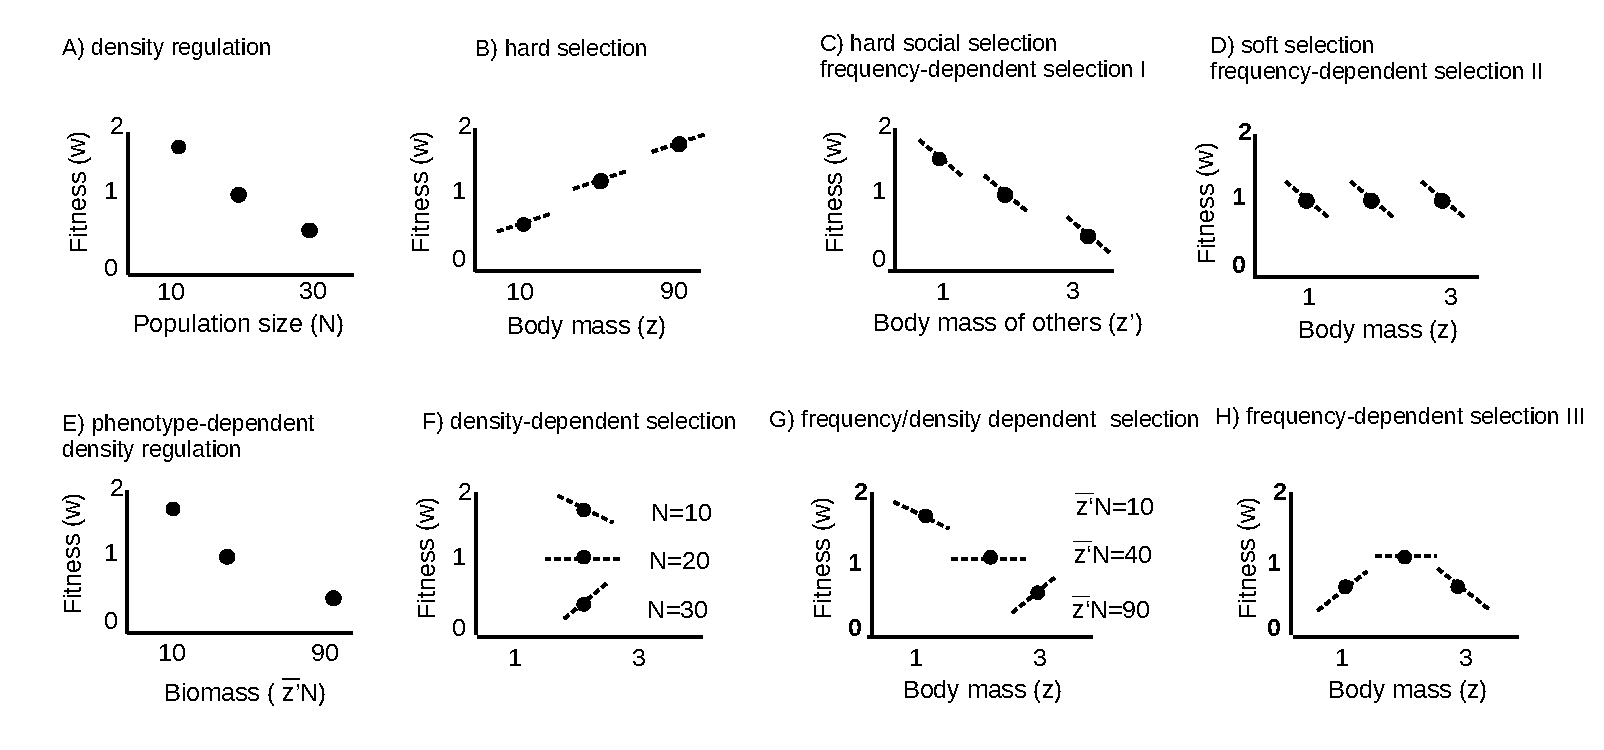
\includegraphics[width=15cm, height=8cm]{Figures/Fig2.pdf}
		\caption{The different social environment effects on the eco-evolutionary dynamics of populations. Here $w$ is used to denote the fitness of individuals, $z$ their phenotypes (e.g. body mass), $N$ the number of individuals in the population, $z'$ the phenotypes of other individuals in the population, and $\bar{z'}$ the average phenotype in the social environment. Black dots represent the average phenotype $\bar{z}$ and fitness $\bar{w}$ for a selection episode, and dashed lines represent the phenotype-fitness relationship within each selection episode. (A) Density regulation, where the number of individuals ($N$) affects the fitness ($w$) of all individuals independent of phenotype. (B) `Hard' selection where the relationship between an individual's phenotype (e.g. body mass) and its own fitness is independent of the social environment (i.e. frequency- and density-independent selection). (C) `Hard' social selection (frequency-dependent selection I), where the phenotype of other individuals (e.g. their body mass) in the population ($z'$) affects individual absolute fitness ($w$), causing the mean phenotype in the social environment to affect population size through its (hard selection) effects on mean fitness. (D) `Soft' social selection (frequency-dependent selection II), where the fitness effects of a phenotype only occur relative to the phenotype and fitness of other individuals with whom it interacts (i.e. dashed lines only). (E) Phenotype-dependent density regulation, where the impact an individual has on the absolute fitness of others depends upon its phenotype (e.g. body mass), and so in this scenario the effect of population size on fitness ($w$) is moderated by the average phenotype in the population ($\bar{z'}N$, e.g. population biomass). (F) Density-dependent selection, where the within-episode (dashed lines) relationship between an individual's phenotype ($z$) and the absolute (black dots) fitness ($w$) depends upon the number of individuals in the population ($N$), but not on the mean phenotype in the population. (G) Density-frequency-dependent selection, where the within-episode relationship between an individual's phenotype ($z$) and its absolute fitness ($w$) depends upon both the number of individuals ($N$) and the mean phenotype (e.g. body mass) in the population ($\bar{z}$). (H) Frequency-dependent selection III, where the relationship between an individual's phenotype and its absolute fitness ($w$) depends upon the mean phenotype in the population ($\bar{z}$), but is independent of the number of individuals in the population ($N$).} \label{fig:selection}
	\end{figure}
	
	\newpage
	\begin{figure} [H]
	\renewcommand{\figurename}{Figure }
		\centering
		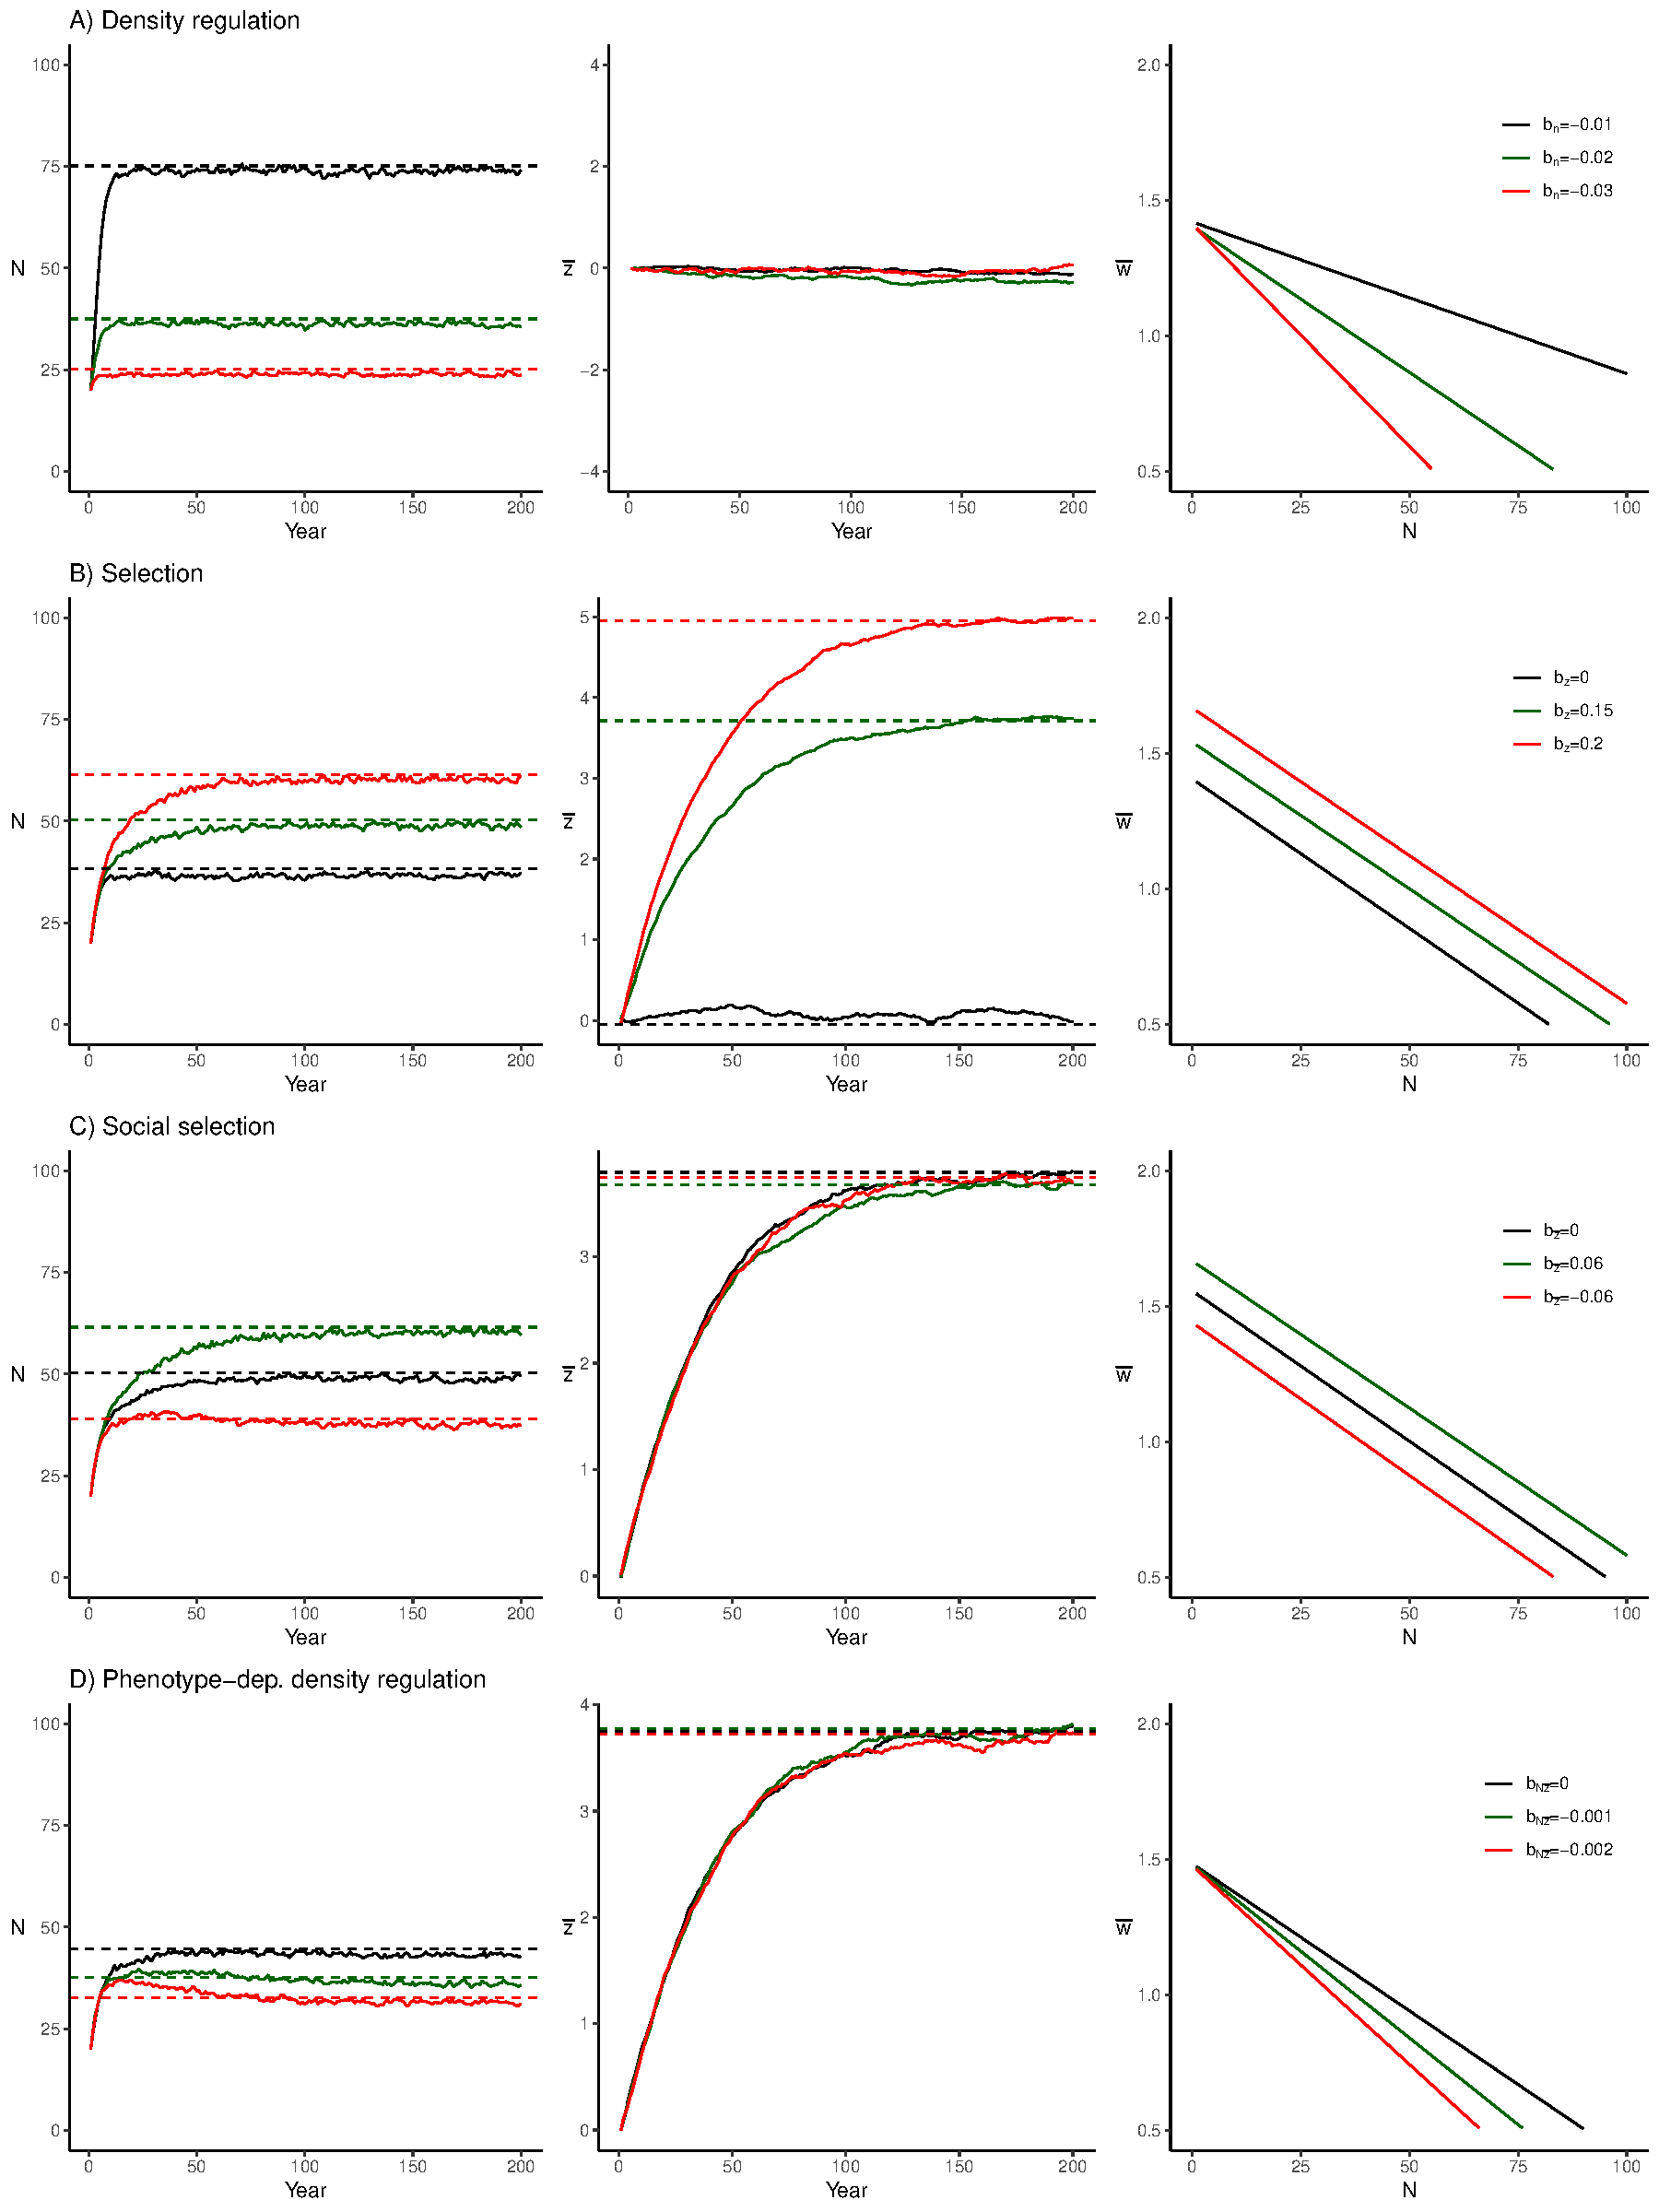
\includegraphics[width=12cm, height=16cm]{Figures/Fig3.pdf}
		\caption{Individual-based simulations results for scenarios 1-4 involving density regulation (A), direct selection on the phenotype (B), `hard' social selection (C) and phenotype-dependent density regulation (D). The left-hand graphs (labelled (i)) show the trajectory of population size (N) each Year until it arrives at its equilibrium, the middle graphs (labelled (ii)) show the trajectory of the mean phenotype ($\bar{z}$) evolving towards its equilibrium, and the right hand graphs (labelled (iii)) show a population's growth rate ($log(\bar{w})$) as a function of population size (N). In each scenario (scenID), we varied a specific parameter while keeping the others constant (see Table 2 for details of all simulation parameters). The values for the parameters that were changed in each case are presented in the legends in the right-hand graphs. Hence the lines of different colours represent different parameter values for each scenario, and stars of each colour are the equilibrium population sizes and mean phenotypes predicted from the statistical model estimates, and the dashed lines represent the predicted trajectories based upon the formulas in Box 3. (A) Scenario 1, density regulation and no selection on the phenotype (i.e. where the average phenotype of the population matches the optimum phenotype and there is no phenotypic evolution - see the flat lines in A(ii)). The strength of density regulation (colour-coded changes in $b_n$ depicted in A(iii)) results in different equilibrium population sizes (A(i)). (B) Scenario 2, `hard' direct selection on the phenotype (e.g. the introduction of a new resource resulting in selection for the ability to exploit it), where the different coloured lines represent different strengths of directional selection ($\beta_{{z}}$) on the phenotype. Evolution gradually shifts the mean phenotypic values closer to the equilibrium phenotype (B(ii)), resulting in different equilibrium population sizes (B(i)), despite the slope of the effect of population size on mean fitness being the same (B(iii)). (C) Scenario 3, `hard' social selection or frequency-dependent selection I, where the mean phenotype of individuals in the social environment affects individual absolute fitness ($\beta_{\bar{z}}$). This affects the equilibrium size of the population (C(i)) because it influences the mean fitness of the population (different elevations in C(iii)), even though the equilibrium phenotype remains the same (C(ii)). (D) Scenario 4, phenotype-dependent density regulation, where the effect of population size on average individual fitness depends upon the mean phenotype in the population ($\beta_{{N\bar{z}}}$). Populations with the same mean phenotype (D(ii)) can have different equilibrium population sizes (D(i)) when the relationship between population size and mean fitness depends on how the mean phenotype modulates the strength of density regulation (i.e. the slopes in D(iii)).}
		\label{fig:sim2}
	\end{figure}
	
	\newpage
	\begin{figure} [H]
	\renewcommand{\figurename}{Figure }
		\centering
		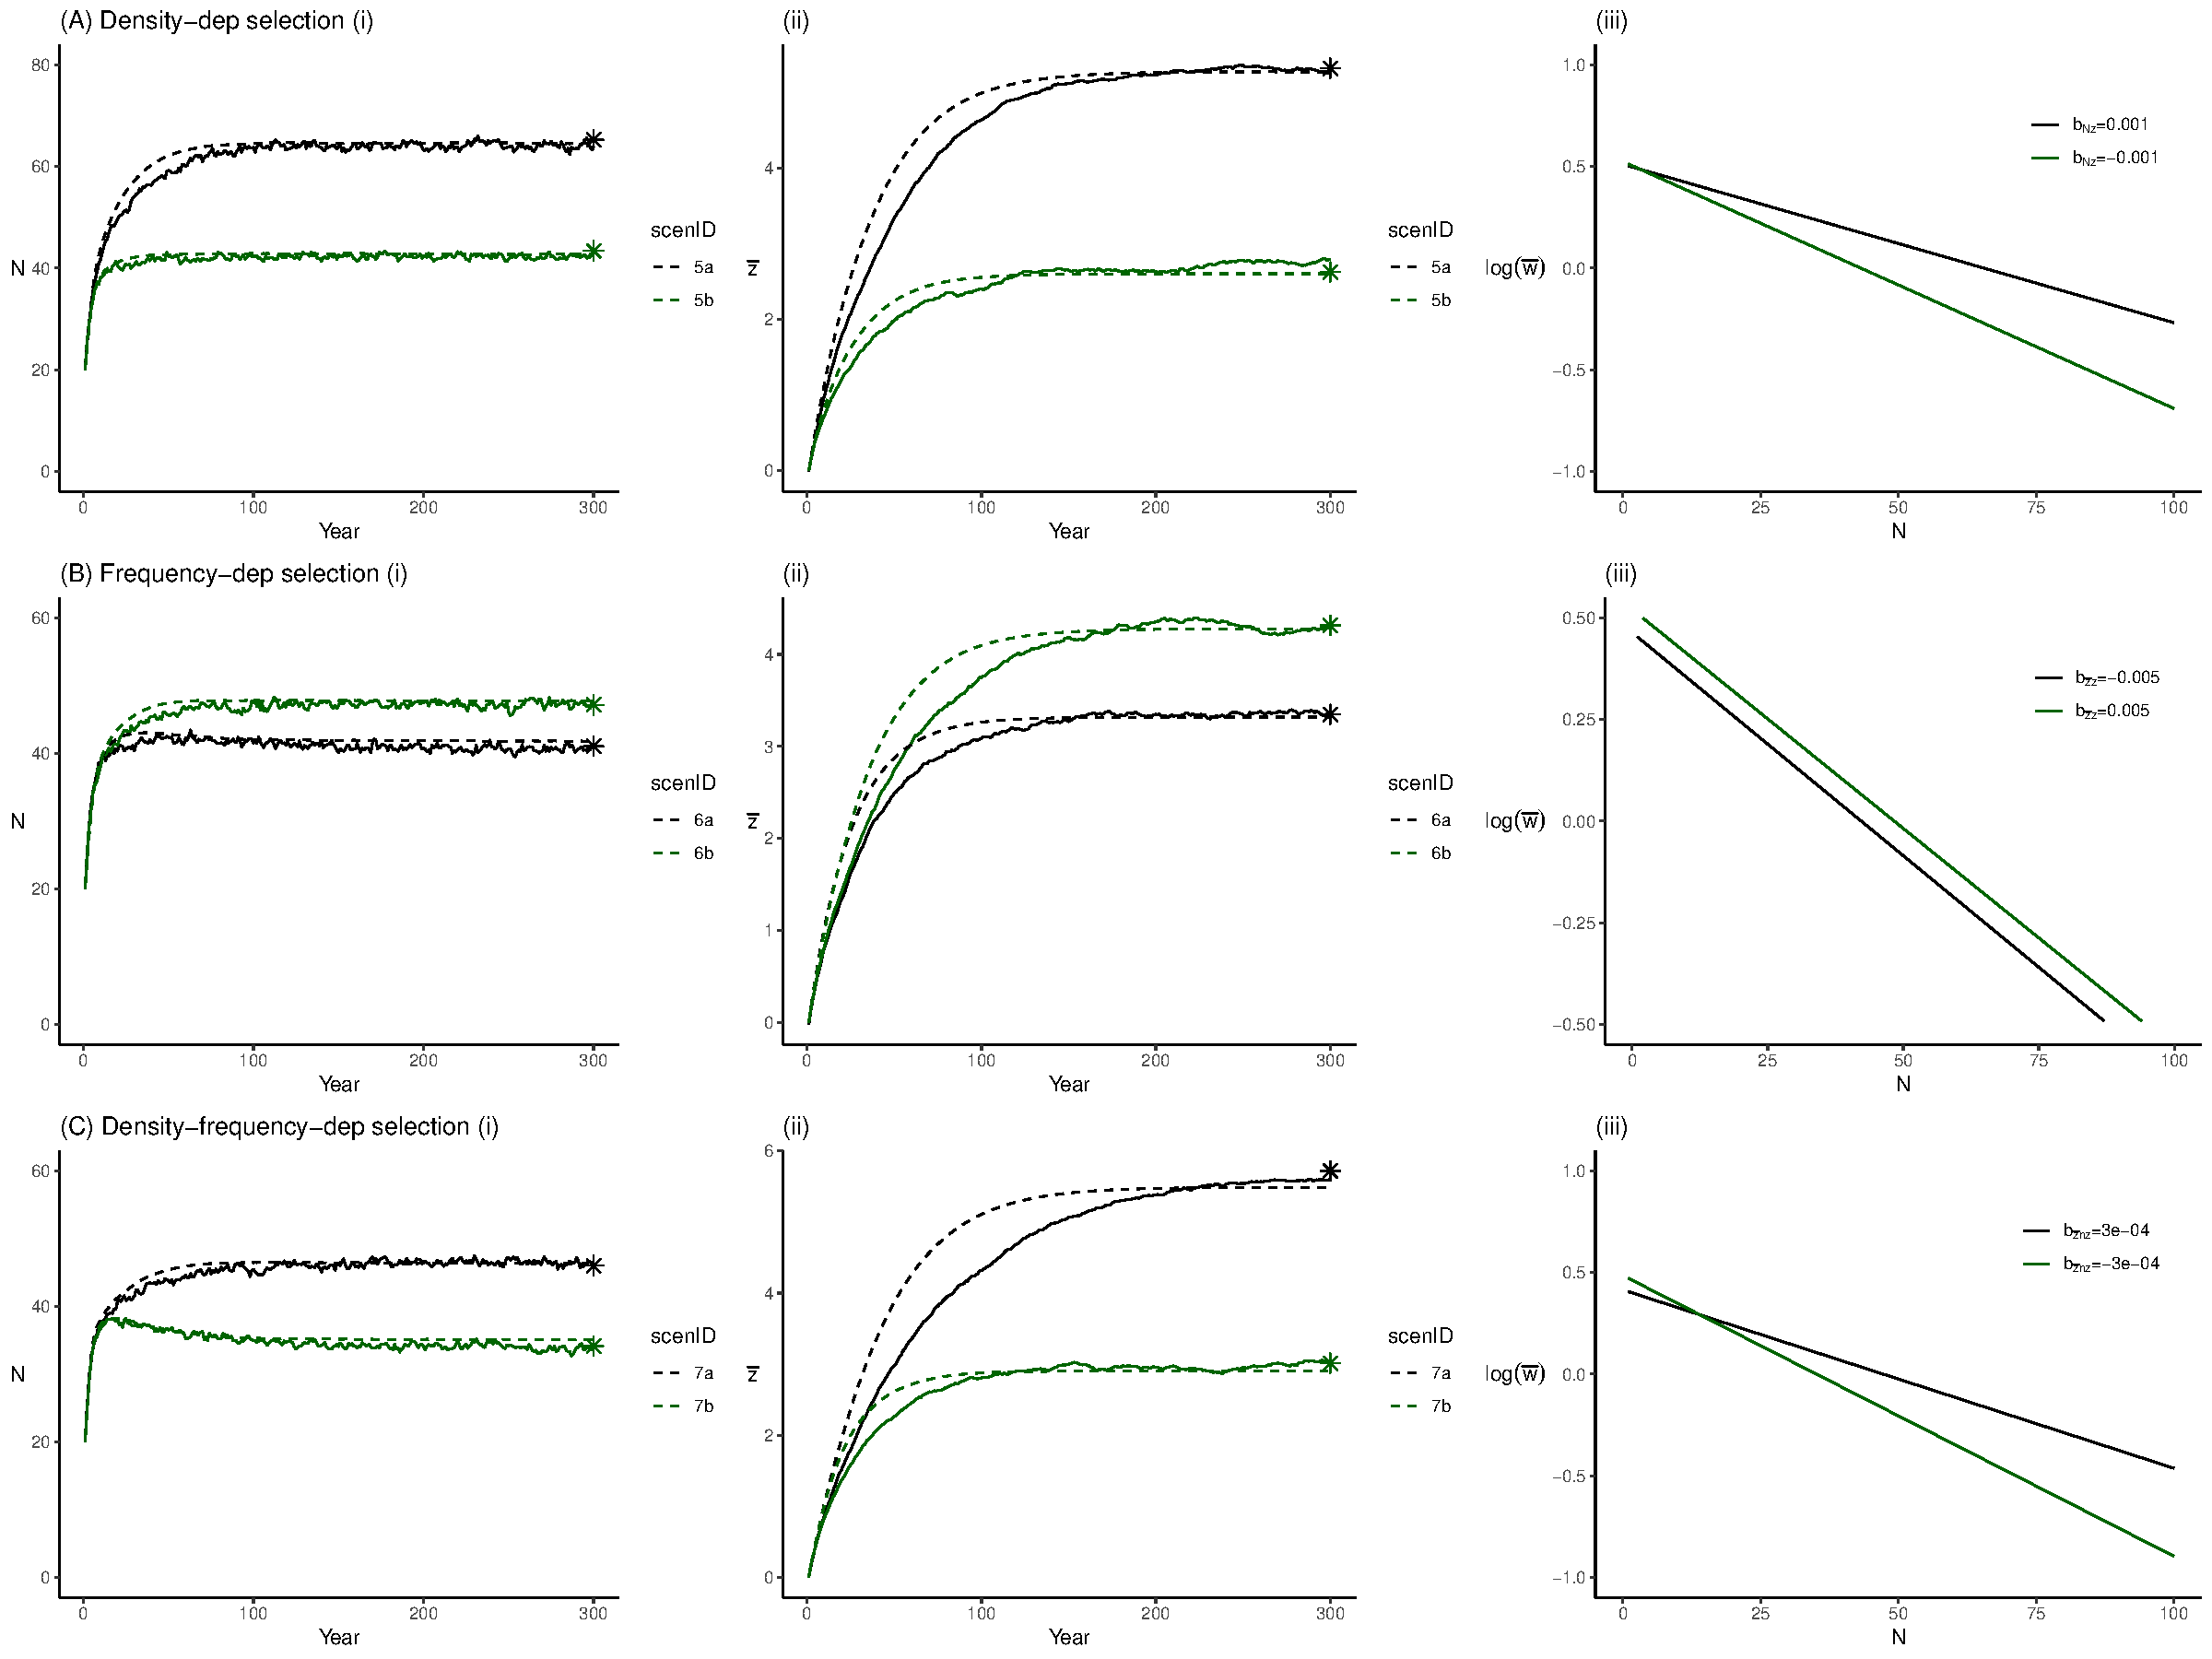
\includegraphics[width=12cm, height=12cm]{Figures/Fig4.pdf}
		\caption{Individual-based simulation results for scenarios 5-7 showing the eco-evolutionary consequences of density-dependent selection (A), frequency-dependent selection II (B), and their interaction (C). As in Figure 2, the left-hand graphs (labelled (i)) show the trajectory of population size over time, the middle graphs (labelled (ii) show the trajectory of the mean phenotype, and the right-hand graphs (labelled (iii)) show the relationship between population density and $log(\bar{w})$. In each scenario (scenID), we varied a specific parameter while keeping the others constant (see Table 2 for details of all simulation parameters). Coloured lines represent different parameter values for each scenario, and stars are the equilibrium population size and mean phenotype predicted from these using the statistical estimates, and dashed lines the expected trajectory predicted by the formulas in Box 3. (A) Scenario 5, density-dependent selection, varies the selection coefficient $\beta_{zn}$ to show how this alters the strength of density regulation (the slopes in A(iii)), with direct consequences for the equilibrium population size (A(i)) and the mean phenotype (A(ii)).(B) Scenario 6, frequency-dependent selection III, varies the coefficient $\beta_{\bar{z}z}$ to demonstrate the consequences for the equilibrium phenotype (B(ii)), as well as for the population size (B(i)) via the effect of the mean phenotype on mean fitness - B(iii). (C) Scenario 7, where frequency- and density-dependent selection interact. Varying the strength of the coefficient ($\beta_{\bar{z}nz}$) determines the interdependence between the mean phenotype (C(ii)) and the equilibrium size of the population (C(i)). The strength of ($\beta_{\bar{z}nz}$) will affect both the mean fitness of a population when its size is very small (the intercepts in C(iii)) and how population size affects the mean fitness of the population (the slopes in C(iii)).} 
		\label{fig:sim3}
	\end{figure}
	
	\newpage
	
	\section{Boxes}
	
	\subsection{Box 1: How social interactions mediate eco-evolutionary feedbacks}
	\setcounter{figure}{0} 
	
	\noindent Figure B.1 depicts the role of social interactions in mediating eco-evolutionary feedbacks through density- and frequency-dependent processes \citep{Engen2020}. Path 1 (p1) shows how the strength of competition for limited resources determines population size through density regulation \citep{Gilpin1973a}. Changes in population size in turn affect density-dependent competition (p2), creating the classic ecological feedback (p1,2) determining the equilibrium size of a population \citep{Travis2013}. If selection is density-dependent (p1,2,3), the size of a population will also have cascading effects on phenotypic selection  \citep{Mueller1997, Boyce1984}. For instance, when populations are large and closer to carrying capacity, investing in somatic growth and competitive behaviours to monopolize resources may be favored. In contrast, when populations are small and resources are abundant, selection may favor smaller individuals that invest in rapid reproduction instead of body size and longer-term competitive ability \citep{Joshi2001, Wright2018, Engen2017}. Density-dependent selection may thus result in the optimal phenotype being dependent upon population size \citep{Anderson1971, Charlesworth1971}. Evolutionary adjustments in the population mean phenotype can, in turn, influence the strength of competitive interactions via the relative frequencies of different phenotypes in the population \citep{Wright1969} (p4,1). Following the example of body size, as competition increases the average individual becomes larger and needs more resources, thus reducing the maximum possible density or carrying capacity of the population \citep{Engen2020}. However, evolution may instead favor social strategies that maximize efficiency of resource use in order to ameliorate the negative fitness effects of competition, potentially increasing the carrying capacity of such populations \citep{macarthur1967theory,  Boyce1984}. When the fitness payoffs from a competitive strategy depend upon the strategy of other individuals in the population, the average phenotype in the population can also influence the optimal phenotype for a given individual. This will cause frequency-dependent selection (see Box 2), further affecting both phenotypic evolution (p4,3) \citep{Heino1998} and population size (p4,3,1) \citep{Svensson2018}. Social interactions thus mediate the feedback between ecological and evolutionary dynamics, linking the evolutionarily stable phenotype with the equilibrium size of a population (p5).
	
	
	\begin{figure}[H]
		\renewcommand{\figurename}{Figure B1.}
		\centering
		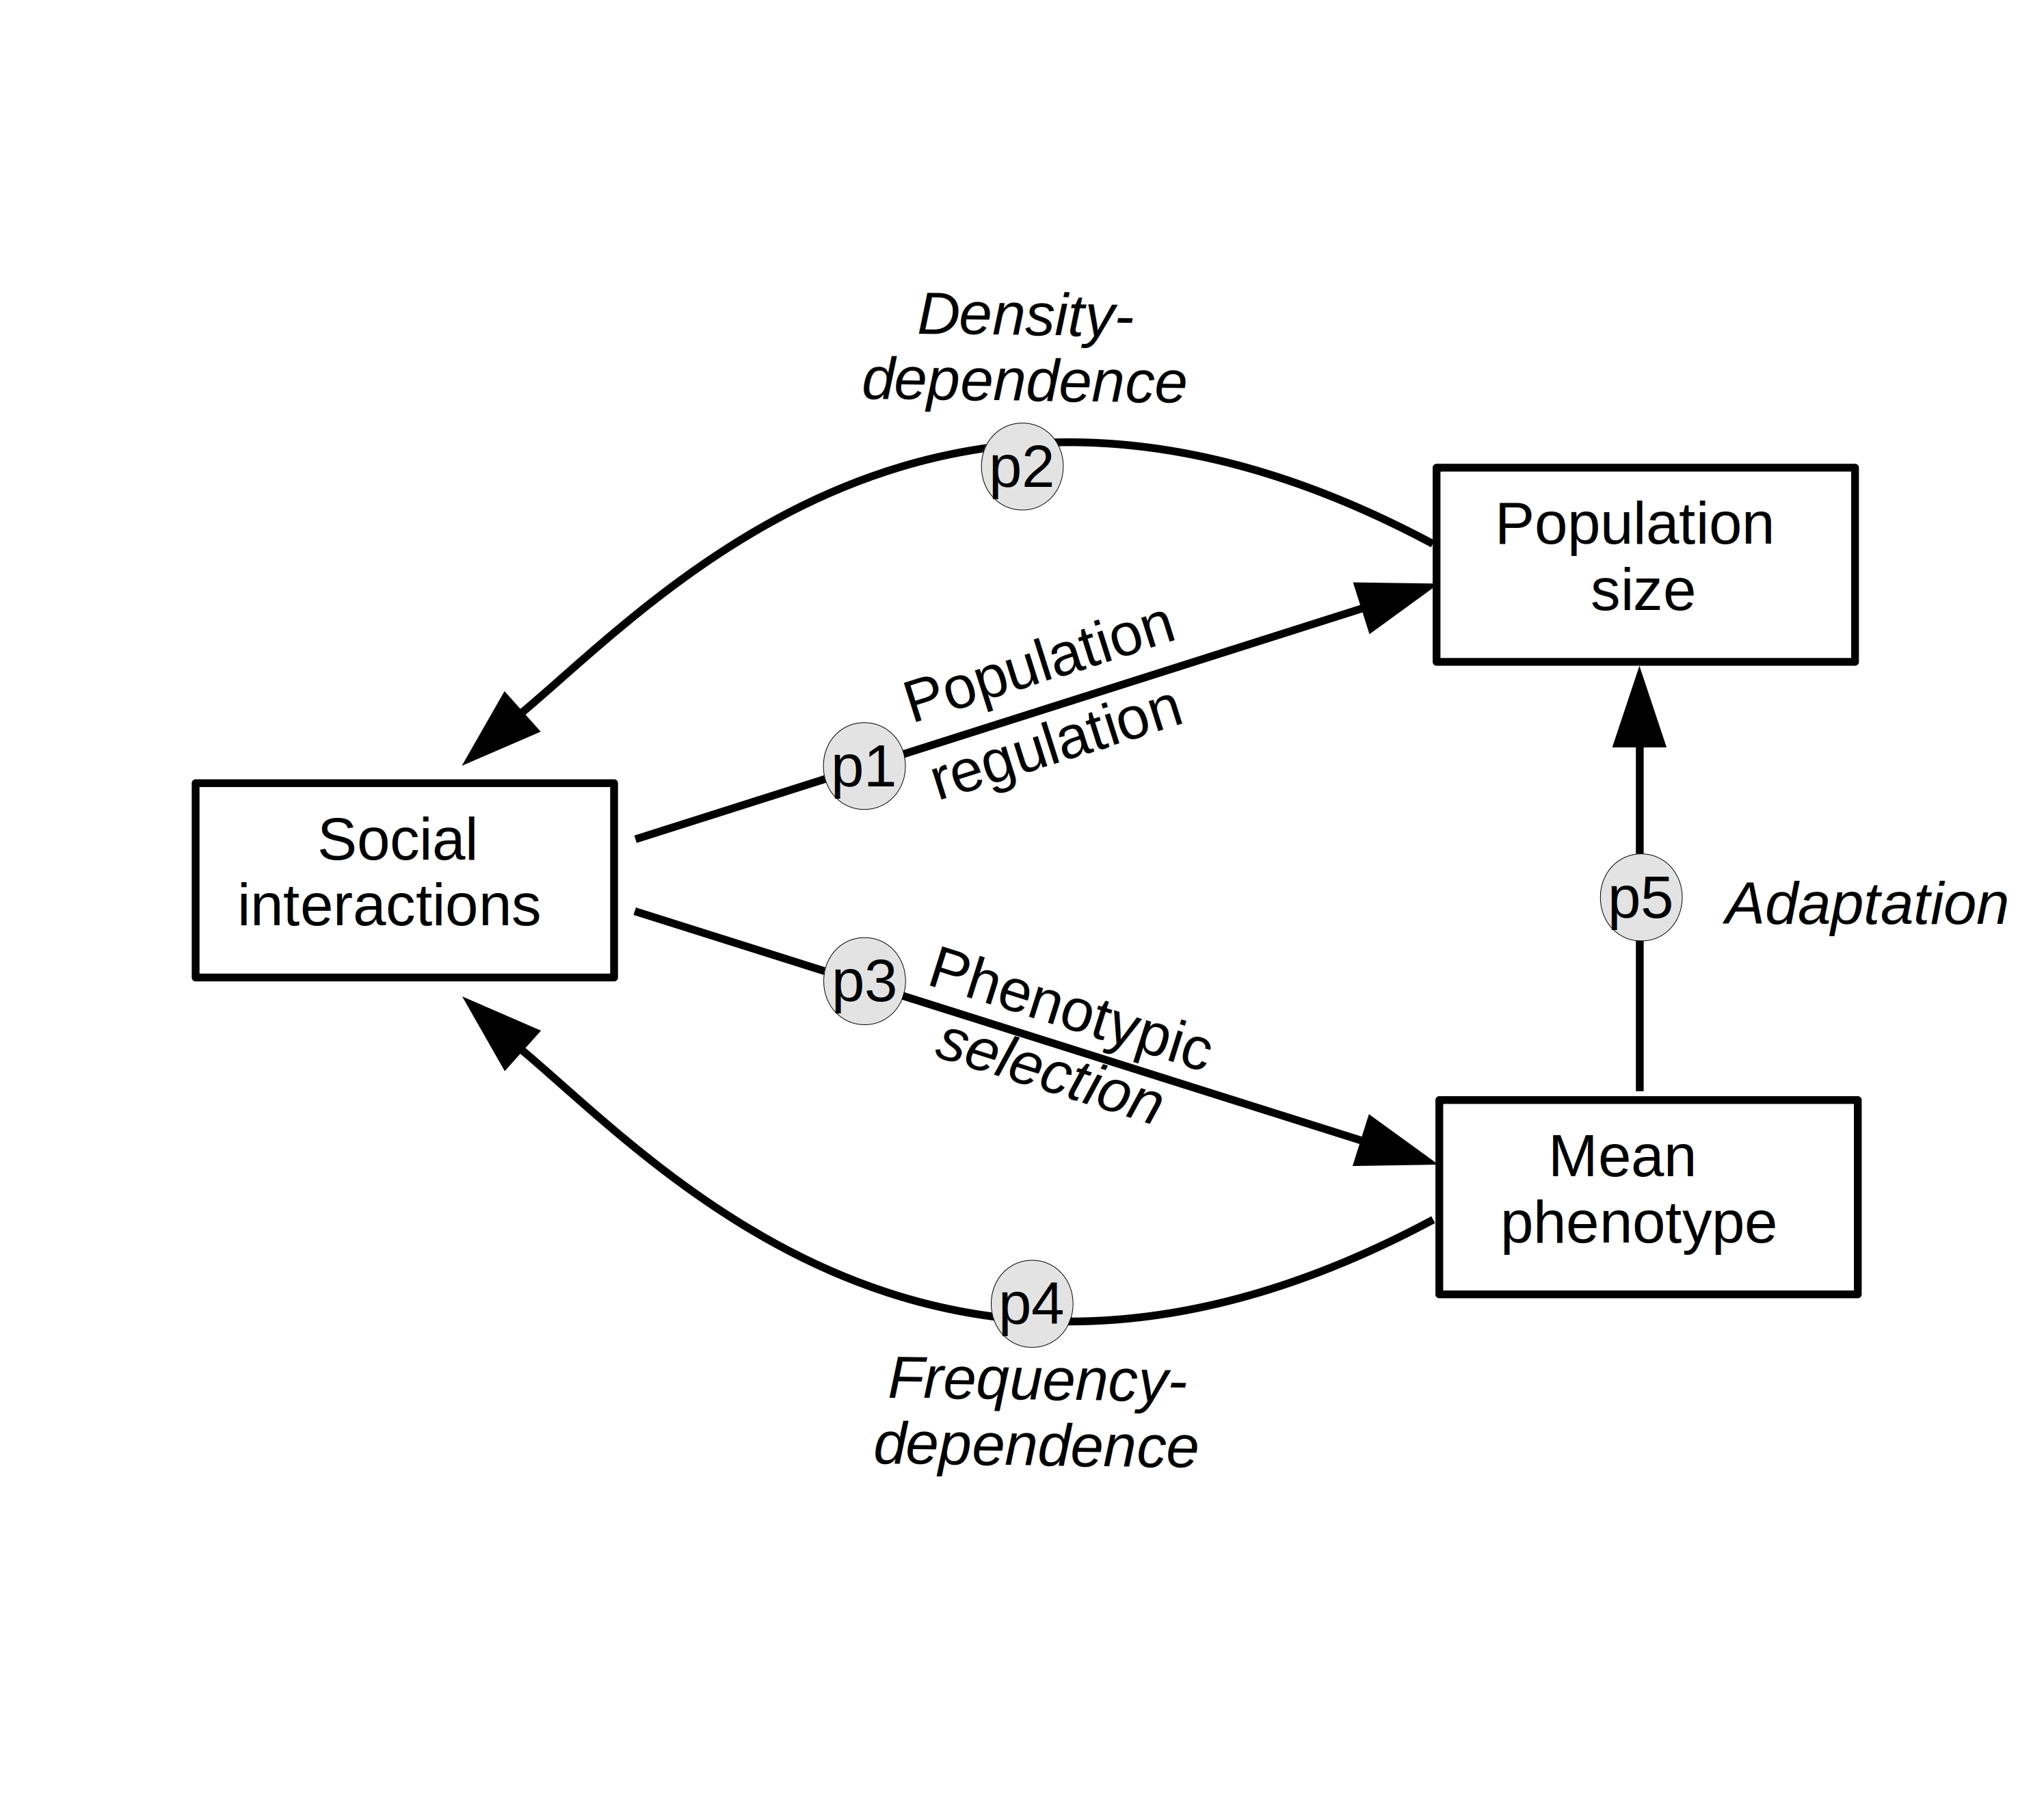
\includegraphics[width=8cm, height=7cm]{Figures/Fig1.jpg}
		\let\nobreakspace\relax
		\caption{Social interactions mediate eco-evolutionary feedbacks}
	\end{figure}
	
	
	\newpage
	\subsection{Box 2: The many types of frequency-dependent selection} 
	\setcounter{figure}{0}    
	\noindent Theoretical models developed in population genetics \citep{Fisher1930, Wright1969}, game theory \citep{MaynardSmith1982, McGill2007, McNamaraLeimar2020} and quantitative genetics \citep{Lande1976, Lande2007, Engen2020} have demonstrated how frequency-dependent selection can affect phenotypic evolution. Classic examples include Fisher's runaway model of sexual selection and the evolution of stable sex ratios \citep{Fisher1930}. However, the term `frequency-dependent selection' is used to describe many different processes and its definition has been extensively discussed, especially in the context of population genetics and the maintenance of polymorphisms \citep{Ayala1974, Gromko1977, Heino1998}. All uses of the term `frequency-dependent selection' have in common that the fitness of a phenotype varies with its frequency in the population. However, it is important to make the distinction between the different types of frequency-dependent selection here, because they can have quite different consequences for phenotypic evolution and population dynamics. Here, we make these distinctions from a statistical perspective, based upon whether the effects of the individual's phenotype and its social environment on its fitness are additive (frequency-dependent selection I), relative (frequency-dependent selection II) or interactive (frequency-dependent selection III).
	
	Frequency-dependent selection I (Figure B2 (i) \& (ii)) refers to scenarios in which the effect of the average phenotype in the social environment and the effect of individual's phenotype on its own fitness have additive effects ($\beta_z \mathbf{z} + \beta_{\bar{z}} \mathbf{\bar{z}}$ ). This situation has been shown to result in maladaptation \citep{Lande1976} and can thus affect population dynamics \citep{Lande2007}. In Figure 1C (main text), we describe such frequency dependence I as `hard' social selection, because the direct effect of an individual's phenotype on its fitness does not change as a function of the average phenotype in the social environment, but the average phenotype affects the absolute fitness of all individuals. 
	
	Frequency-dependent selection II (Figure B2 (iii) \& (iv)) describes scenarios in which the effect of a phenotype on fitness is relative to the average phenotype in the social environment ($\beta_z [z-\bar{z}]$). This type of frequency-dependent selection includes `soft' selection \citep{Wallace1975, Bell2021}. This can be thought of as a zero-sum game, where a fitness gain of one individual or phenotype results directly in a fitness loss in another, and thus soft selection has no net effect on the mean fitness in the population. Frequency-dependent selection II can also be related to more narrow definitions that require negative frequency-dependent selection to result in the stable coexistence of polymorphisms (i.e. where the fitness of a phenotype decreases with its relative frequency in the population). This process was at the center of early developments of the concept of frequency-dependent selection in game theory and population genetics \citep{MaynardSmith1982, McGill2007, Gromko1977, Ayala1974, Heino1998}. In a quantitative genetic framework, it can be formulated as a type disruptive selection \citep{Burger2004}, were the effects of a phenotype depends on the absolute deviation from the average phenotype in the population ($[z-\bar{z}]^2$). 
	
	Frequency-dependent selection III (Figure B2 (v) \& (vi), and Figure 1G main text) consists of scenarios in which an individual's phenotype interacts with the average phenotype of its social environment to affect its fitness ($\beta_{z\bar{z}} \mathbf{\bar{z}z}$). This results in a warped fitness surface where the direct effect of a phenotype on fitness changes with the average phenotype in the social environment \citep{Araya-Ajoy2020}. This may represent a type of balancing selection \citep{Gromko1977}. For instance, in a scenario where the mean population phenotype becomes larger then individuals with a smaller phenotype will have an advantage, but as the mean phenotype becomes smaller individuals with a larger phenotype will have an advantage (see Figure B2 (vi)).
	
	\begin{figure}[H] 
		\renewcommand{\figurename}{Figure B2.}
		\centering
		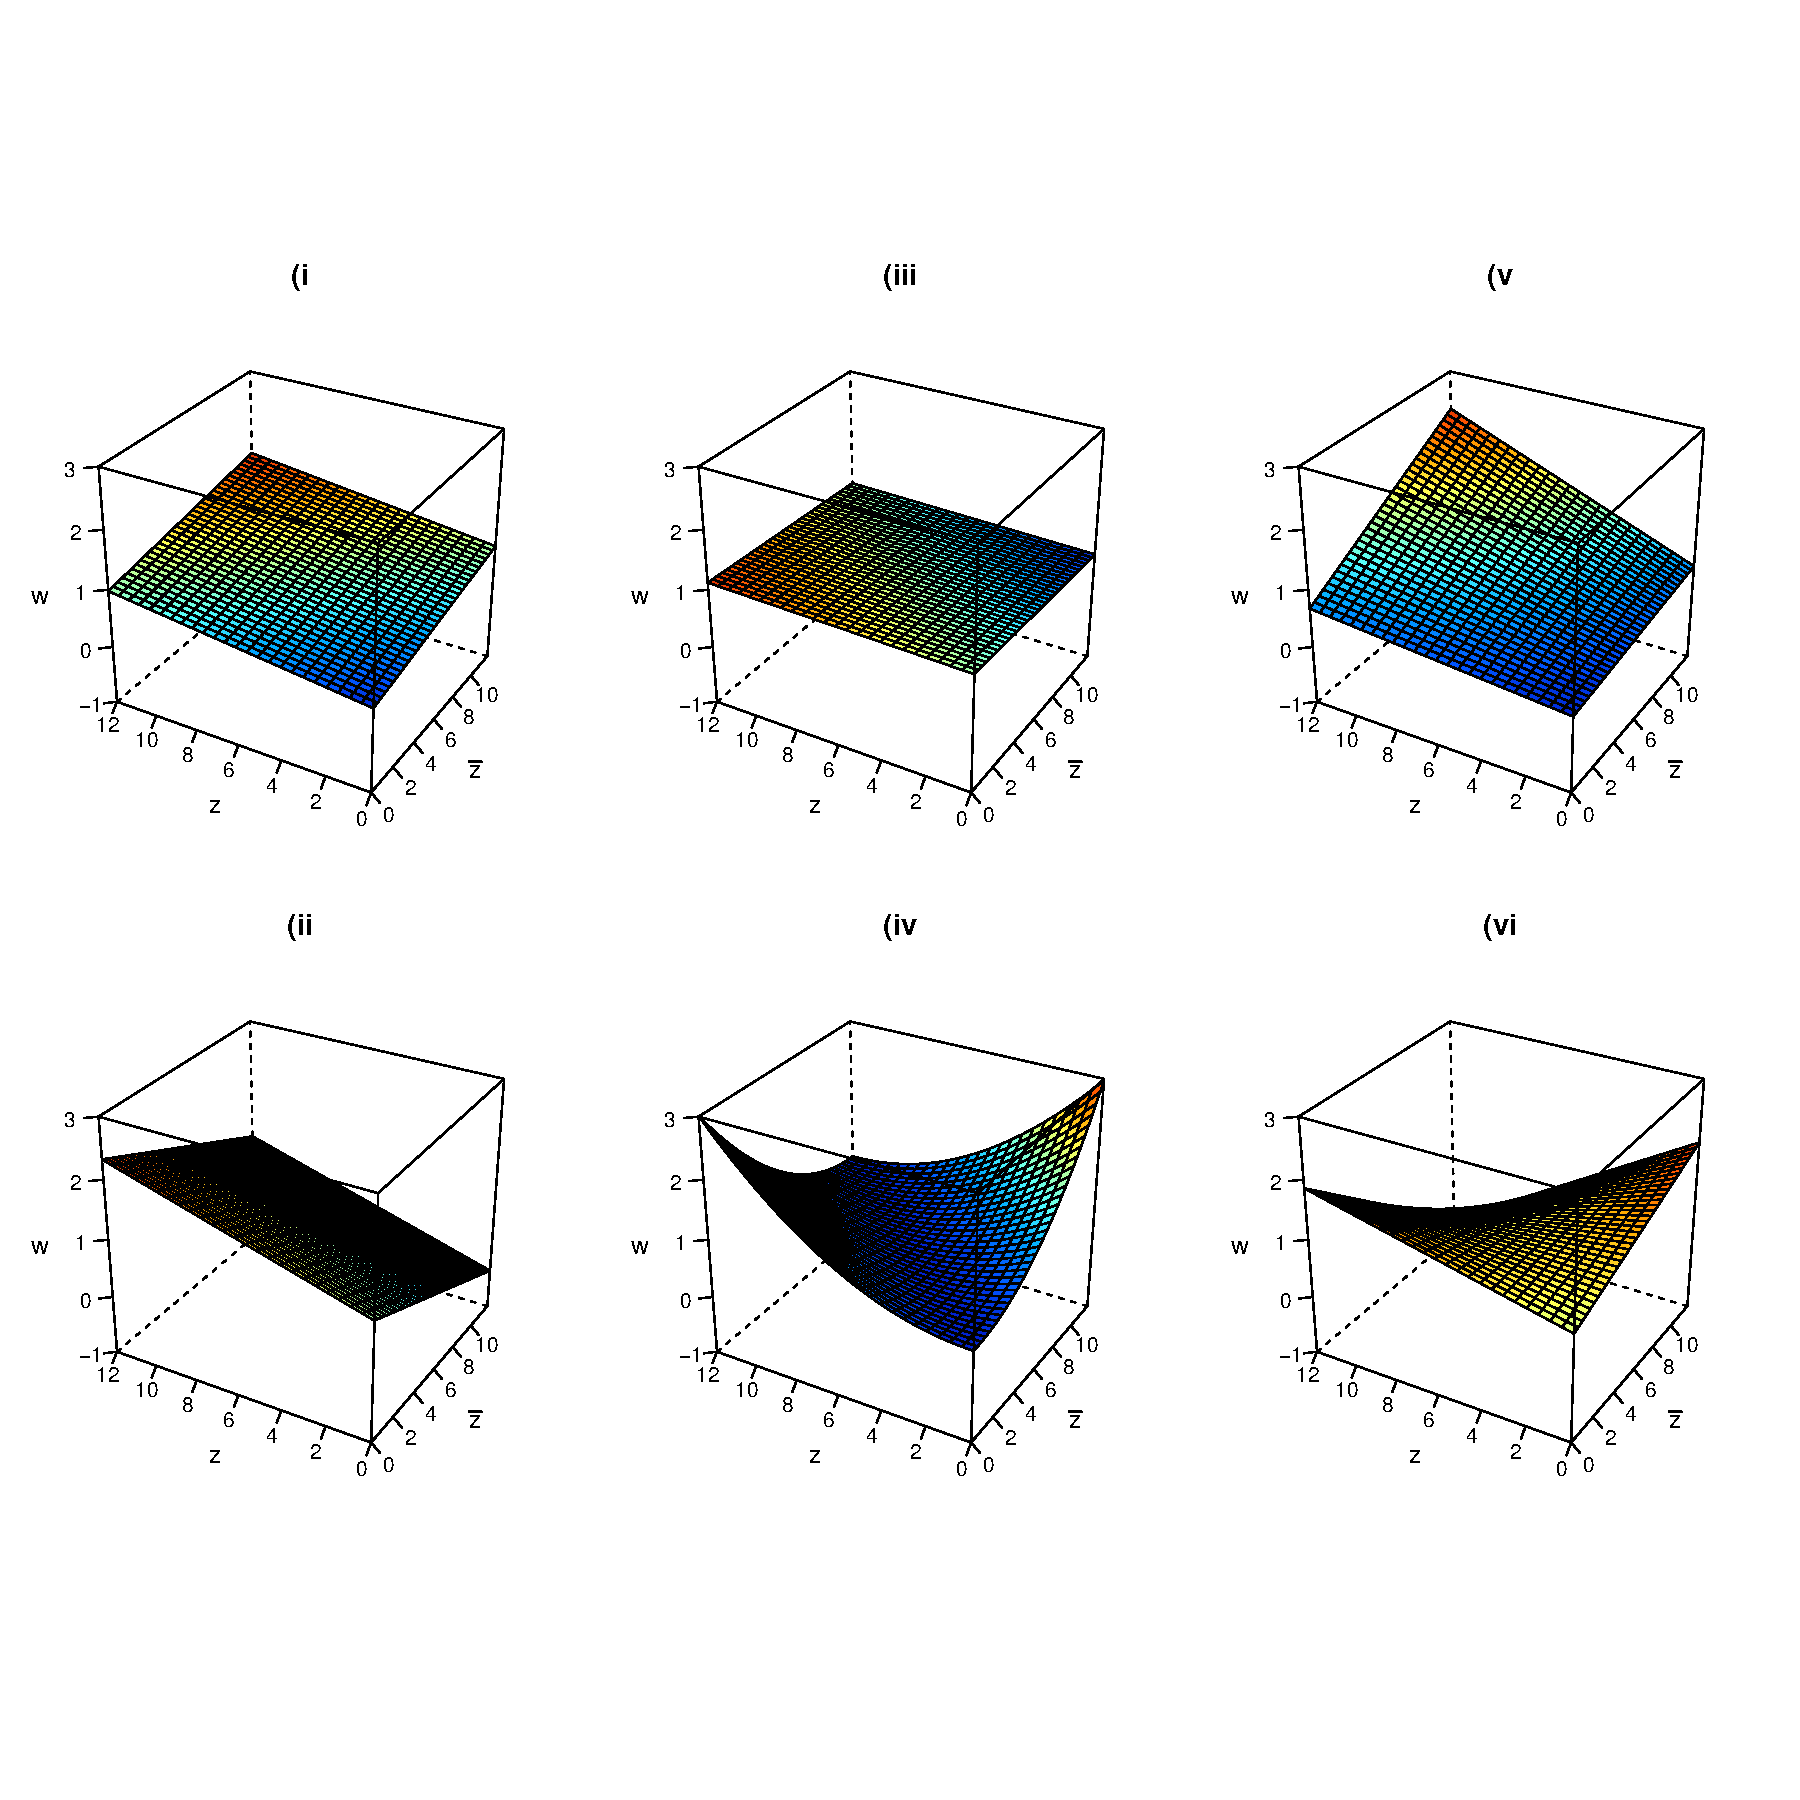
\includegraphics[width=14cm, height=14cm]{Figures/Box2.pdf}
		\let\nobreakspace\relax
		\caption{Fitness surfaces for different types of frequency-dependent selection. The left-hand panels represent scenarios of (i) positive and (ii) negative frequency dependence I, in which the effects of an individual's phenotype and that of its social environment have additive effects on its fitness ($\beta_z \mathbf{z} + \beta_{\bar{z}} \mathbf{\bar{z}}$). The middle panels (iii) and (iv) represent scenarios of frequency-dependent selection II, in which the effects of an individual's phenotype on its fitness are relative to the average phenotype in its social environment, with (iii) a scenario of positive selection for having a higher phenotypic value than that of the average individual in the social environment ($z-\bar{z}$), and (iv) a scenario of negative frequency-dependent selection (and the evolution of polymorphisms) in which the effects of the phenotype depend upon its absolute deviation from the mean phenotype in the social environment ($(z-\bar{z})^2$). The right-hand panels represent scenarios of (v) positive and (vi) negative frequency dependence III, in which an individual's phenotype interacts with that of its social environment to affect its fitness ($\beta_{z\bar{z}} \mathbf{\bar{z}z}$), such that the fitness function depends upon the mean phenotype in the social environment. See Box 2 text for more detail.}
		
	\end{figure}
	
\subsection{Box 3: Analytical approximations for the expected evolutionary change}
	\setcounter{table}{0}    
	
We can approximate the selection gradients that will determine the expected evolutionary change in the mean phenotype of the population based upon the log-linear effects of the phenotype on fitness ($w$). It is important to keep in mind here that the we are modeling several episodes of selection together, where both the mean fitness of the population and the selection gradients fluctuate due to changes in the number of individuals in the population and its mean phenotype. The different individual-based simulation (IBS) scenarios assume that fitness ($w$) is dependent upon an individual's phenotype ($z$), population size ($n$) and the mean phenotype of the population ($\bar{z}$), and that these effects are caused solely by their influence on recruit production. The fitness function can thus be written as:  		

\begin{equation}
 w(\bm z; N,\bar{\bm z}).  \tag{B3.1}\label{B32}
\end{equation}

The models presented in the main text assume linear effects of phenotypes and population size on log fitness, $\ln w$, which can thus be thought of as a population growth rate measure ($v$). Therefore, the underlying fitness model is: $\ln w=v(\bm z; N,\bar{\bm z}).$ At a given value of $\bar{z}$ and $n$, the population growth rate fluctuates around the expected value $\bar{v}=\ln \bar{w}$, which is the expected value of $v$ with respect to variation of $z$ in the population within an episode of selection. The deviation $\Delta v$ of each phenotype's expected growth rate $v$ from the population mean growth rate ($\bar{v}$) in a give episode of selection can thus be expressed as:
		\begin{equation}
\Delta v=v-\bar{v}. \tag{B3.2}\label{B33} 
	    \end{equation}
We can infer an individual's fitness ($w$) from its growth rate ($v$) using a first order approximation, where 

\begin{equation}
 w=e^{\bar{v}+\Delta v}\approx \bar{w}+\bar{w}\Delta v . \tag{B3.3}\label{B34} 
\end{equation}	
 	
\noindent The corresponding approximation to the fitness function at $\bar{z}$ and $N$ can thus be expressed as:
 \begin{equation}
 w(z,\bar{z},n)=\bar{w} + \bar{w} \Delta v(z,n, \bar{z}),  \tag{B3.4}\label{B35} 
 \end{equation}

\noindent where the expected population size in the next time step is equal to $ne^{\bar{v}}$, and the relationship between the phenotype and relative fitness can then be expressed as:

\begin{equation}
\frac{w}{\bar{w}}= \frac{\bar{w} + \bar{w} \Delta v(z,n, \bar{z})}{\bar{w}}=1 + \Delta v(z,n, \bar{z}). \tag{B3.5}\label{B36} 
\end{equation}

The response to selection is now given by the gradient of mean relative fitness taken only with respect to the $\bar{z}$ resulting from averaging over the distribution of $z$ in the population. The gradient of $ \Delta v$ can be thought of as the selection gradient for a given episode (times step) where the population size is $n$ and the mean phenotype $\bar{z}$. Note that log fitness is very similar to dividing fitness by its mean, and thus the model involving $v$ is a very close approximation to a model of relative fitness ($\frac{w}{\bar{w}}$). The selection gradient for a given episode can thus be approximated based upon the estimates ($\beta$) from the log-linear effects on fitness (e.g. Equation 19 in the main text). The formulas for each scenario are presented in Table B3.1. The selection gradient will vary as a function of how far the mean phenotype of the populations is from the optimum phenotype (i.e. S2-7). While under density- and frequency-dependent selection it will depend upon $n$ and $z$, respectively (S5 \& S6), and in the most complex scenario we have sketched in the main text, it can depend upon both (S7). Since the gradient of $\Delta v$ is the same as that of $\bar{v}$, we can write this as: 

\begin{equation}
 \Delta \bar{z}=h^2P \nabla \bar{v}(\bar{z},N,\bar{z}^*), \tag{B3.6}\label{B37} 
\end{equation}

\noindent where $h^2$ is the heritability, $P$ is the phenotypic variance, and the gradient is taken with respect to $\bar{z}$. Note that we insert $\bar{z}^*=\bar{z}$ to clarify that the gradient is with respect to the direct effect of the phenotype on fitness. This formula can be used to predict the expected evolutionary change in our simulation, because fitness variation is solely caused by effects on recruit production. For the analytical approximation of the results of the IBS, see Appendix 1.

\bigskip  
	
\begin{table}
	\renewcommand{\tablename{Table B3.}}
	\begin{singlespace}
		\begin{flushleft} 
			\begin{tabular}{ p{19mm} p{46mm} p{53mm} p{27mm} } 
				\hline
				
				     \textbf{Scenario} & \textbf{Growth rate} ($\bm{\bar{v}}$) &  \textbf{Growth rate deviations} ($\bm{\Delta v}$) &  \textbf{Gradient} ($\bm{\nabla \bar{v}}$)   \\ [2pt]
				
				1.   $w(n)$ & $\beta_n n$ & - &- \\ [2pt]
				
				2.   $w(z,n)$ &  $\beta_n n + \beta_z \bar{z} + \beta_q \bar{z^2} $ & $\beta_z (z-\bar{z}) + \beta_q (z^2-\bar{z^2})$  &$ \beta_z  + 2\beta_q \bar{z}$  \\ [2pt]
				
				3.  $w(z,n, \bar{z})$ &  $\beta_n n + (\beta_z + \beta_{\bar{z}})\bar{z} + \beta_q \bar{z^2} $ &$\beta_z (z-\bar{z}) + \beta_q (z^2-\bar{z^2})$& $ \beta_z  + 2\beta_q \bar{z}$  \\ [2pt]
				
				4.   $w(z,n, \bar{z})$ &  $(\beta_n + \beta_{n\bar{z}}\bar{z}) n + (\beta_z + \beta_{\bar{z}})\bar{z} + \beta_q \bar{z^2} $ & $\beta_z (z-\bar{z}) + \beta_q (z^2-\bar{z^2})$ & $ \beta_z  + 2\beta_q \bar{z}$  \\ [2pt]
				
				5.  $w(z,n)$ &  $(\beta_n + \beta_{n\bar{z}}\bar{z}) n + \beta_z\bar{z} + \beta_q \bar{z^2}$ &$\beta_z (z-\bar{z}) + \beta_q (z^2-\bar{z^2}) + \beta_{nz} (zn-\bar{z}n)$  & $ \beta_z  + 2\beta_q \bar{z} + \beta_{nz}n$  \\ [2pt]
				
				6.  $w(z,\bar{z})$ &  $\beta_n n + \beta_z\bar{z} + \beta_q \bar{z^2} + \beta_{z\bar{z}}\bar{z}^2 $ &$\beta_z (z-\bar{z}) + \beta_q (z^2-\bar{z^2}) +  \beta_{z\bar{z}} (zz-\bar{z}^2)$  & $ \beta_z  + 2\beta_q \bar{z} + \beta_{z\bar{z}}\bar{z}$  \\ [2pt]
				
				7.  $w(z,n, \bar{z})$ &  $ n(\beta_n + \bar{z}[\beta_{n\bar{z}} + \beta_{zn} + \beta_{zn\bar{z}}\bar{z}]) + \bar{z}(\beta_z + \beta_{\bar{z}} + \beta_{z\bar{z}}\bar{z}) + \beta_q \bar{z^2}   $ &$\beta_z (z-\bar{z}) + \beta_q (z^2-\bar{z^2}) +  \beta_{z\bar{z}} (z\bar{z}-\bar{z}^2)  + \beta_{nz} (zn-\bar{z}n) +  \beta_{zn\bar{z}}(zn\bar{z}-n\bar{z}^2)$  & $ \beta_z  + 2\beta_q \bar{z} + \beta_{z\bar{z}}\bar{z} + (\beta_{nz} +\beta_{zn\bar{z}}\bar{z})n$  \\ [2pt]
				\hline
				
			\end{tabular}
			\caption{Equations to estimate the predicted average growth rate for each episode of selection in the different scenarios $\bar{v}$, the expected deviation for each phenotype from the population growth rate ($\Delta v$) and the gradient relating the phenotype with its fitness within each episode of selection ($\nabla \bar{v}$). These equations can then be used to predict the fluctuations in mean fitness and thus the effects on population size, as well as the expected changes in mean phenotype in the population based on the equations presented in the text of Box 3. For the definitions of parameters see Table 1 in the main text.}
		\end{flushleft} 
	\end{singlespace}
\end{table}
\bigskip
	\newpage

	\section{Supplementary Material}
		\setcounter{table}{0}    
		\subsection{Appendix 1: Estimating the selection gradients for a given episode}
		The individual-based simulation (IBS) assumes that all individuals had the same underlying survival probability $\bar{p}$, and that the effects of an individual's phenotype ($z$), population size ($n$) and the mean phenotype in the population ($\bar{z}$) are realized through effects on recruit production $r$. The underpinning equations for the vital rates of individuals in the population are:
		
		\begin{subequations} 
			\begin{gather}
			\bm{r}\sim Poisson(e^{b_{0} + b_{n} \bm{n} + b_{z} \bm{z} + b_{q} \bm{z^2} + b_{\bar{z}} \bm{\bar{z}} + b_{n \bar{z}} \bm{n\bar{z}} + b_{z\bar{z}}  \bm{z\bar{z}} + b_{zn}  \bm{zn} + b_{zn \bar{z}} \bm{zn\bar{z}}+  \bm{e}}), \tag{A1.1a} \\
			\bm{s}\sim Bern(\frac{1}{e^{\bar{p}}}). \tag{A1.1b}
			\end{gather}
		\end{subequations}
		
		\noindent Here $b_0$ is the average log recruit production in the population when it is very small. Population size effects on the log number of recruits is described by the density regulation coefficient $b_{n}$. An individual's recruit production can be affected by its own phenotype as a function of the linear ($b_z$) and quadratic ($b_q$) effects of the phenotype on fitness. The number of recruits produced by an individual can also depend upon the (average) phenotype ($\bar{z}$) of the individuals in the population modulated by the coefficient $b_{\bar{z}}$. Furthermore, the average phenotype in the population can also modulate the strength of density regulation as a function of the interaction coefficient $b_{n\bar{z}}$. The optimal phenotype can depend upon the number of individuals in the population ($b_{zn}$) and also upon the mean phenotype in the population ($b_{z\bar{z}}$). Ultimately, the relationship between phenotype and fitness may also depend upon an interaction between the number of individuals and the phenotype of the average individual in the population ($b_{zn\bar{z}}$).
		
		We can approximate how the log-linear effects of the phenotype and population size on recruit production affect population dynamics and the patterns of selection through its effects on individual fitness $w$. The different simulation scenarios assume that fitness ($w$) is dependent upon an individual's phenotype $z$, population size $\bar{z}$ and the mean phenotype of the population ($\bar{z}$). This is can be written as:
		  		
		\begin{equation}
		w(\bm z; N,\bar{\bm z})= s+ r(\bm z; N,\bar{\bm z}),  \tag{A1.2}
		\end{equation}
		
		\noindent where	$s$  is the survival of an individual and $r$ is the number of recruits produced. In this IBS, we have assumed a linear model with $\rho$ being equal to $\ln r$. Therefore, the underlying model of the simulation is $r=\rho(\bm z; N,\bar{\bm z}).$
		
		At a given value of  $\bar{z}$ and $n$ for the IBS, the mean number of recruits fluctuates around the expected value $\bar{v}=\ln \bar{r}$, which is the expected value of $\rho$ with respect to variation in $z$ in the population. The deviation of each phenotype's expected log recruit production, $v$, can thus be expressed as:
		\begin{equation}
		\Delta \rho=\rho-\bar{\rho}. \tag{A1.3} 
		\end{equation}
		The first order approximation to $r$ is thus: 
		
		\begin{equation}
		r=e^{\bar{\rho}+\Delta \rho}\approx \bar{r}+\bar{r}\Delta \rho . \tag{A1.4}\label{B34} 
		\end{equation}	
		
		The corresponding approximation to the fitness function at $\bar{z}$ and $n$ is now: 
		\begin{equation}
		w(z,\bar{z},n)=s+\bar{r} + \bar{r} \Delta \rho(z,n, \bar{z}),  \tag{A1.5}\label{B35} 
		\end{equation}
		
		and since the mean fitness at $\bar{z}$ and $n$ is $\bar{w}=s + r$, the relative fitness is: 
		\begin{equation}
		\frac{w}{\bar{w}}=1+\frac{r}{s+r}\Delta \rho(z,n,\bar{z}). \tag{A1.6}\label{B36} 
		\end{equation}
		
		The response to selection is now given by the gradient of mean relative fitness taken only with respect to $\bar{z}$, obtained by averaging across the distribution of $z$ in the current population. Since the gradient of $\Delta \rho$ is the same as that of $\rho$ we can write this as: 
		\begin{equation}
		\Delta \bar{z}=h^2P\frac{r}{s+r}\nabla \bar{\rho}(\bar{z},N,\bar{z}^*), \tag{A1.7}\label{B37} 
		\end{equation}
		
		\noindent where $h^2$ is the heritability, $P$ is the phenotypic variance, and the selection gradient is taken with respect to $\bar{z}$. Note that we insert $\bar{z}^*=\bar{z}$ to clarify that the selection gradient is with respect to the direct effect of the mean phenotype on fitness. 
		
		Notice that at equilibrium defined by $\bar{w}=1$, we have $\bar{r}=1-s$ giving: 
		\begin{equation}
		\Delta \bar{z}=h^2P\nabla \bar{\rho}(\bar{z},n,\bar{z}^*)/T, \tag{A1.8}\label{B38} 
		\end{equation}
		
		\noindent where $T=1/(1-s)$ is the generation time measured at equilibrium. For a fluctuating population, however, the factor $\bar{r}/(s+\bar{r})$ is a function of $\bar{z}$ and $n$, and therefore fluctuates around $T$. 
		In a finite population, with zero mean and variance in $\Delta \bar{z}$ during a generation, the genetic drift is  $h^2P/(n)$, and during a time step $h^2P/(nT)$, giving:
		\begin{equation}
		\Delta \bar{z}=h^2P\frac{\bar{r}}{s+\bar{r}}\nabla \bar{\rho}(\bar{z},N,\bar{z}^*)+\sqrt{h^2P/(NT)}U_{drift}, \tag{A1.9}\label{B39} 
		[\end{equation} 
		
		where $U_{drift}$ is a standard normal variable.  
		
		\begin{table} [h]
		\renewcommand{\tablename{Table A.}}
			\begin{singlespace}
				\begin{flushleft} 
					\begin{tabular}{ l  p{45mm} p{52mm} p{30mm} } 
						\hline
						
						\textbf{Scenario}   &  \textbf{Ln mean recruits} ($\bm{\bar{\rho}}$) &  \textbf{Ln recruits deviations} ($\bm{\Delta \rho}$) &  \textbf{Gradient} ($\bm{\nabla \bar{\rho}}$)   \\ [2pt]
						
						1.   $w(n)$ & $b_n n$ & - &- \\ [2pt]
						
						2.   $w(z,n)$ &  $b_n n + b_z \bar{z} + b_q \bar{z^2} $ & $b_z (z-\bar{z}) + b_q (z^2-\bar{z^2})$  &$ b_z  + 2b_q \bar{z}$  \\ [2pt]
						
						3.  $w(z,n, \bar{z})$ &  $b_n n + (b_z + b_{\bar{z}})\bar{z} + b_q \bar{z^2} $ &$b_z (z-\bar{z}) + b_q (z^2-\bar{z^2})$& $ b_z  + 2b_q \bar{z}$  \\ [2pt]
						
						4.   $w(z,n, \bar{z})$ &  $(b_n + b_{n\bar{z}}\bar{z}) n + (b_z + b_{\bar{z}})\bar{z} + b_q \bar{z^2} $ & $b_z (z-\bar{z}) + b_q (z^2-\bar{z^2})$ & $ b_z  + 2b_q \bar{z}$  \\ [2pt]
						
						5.  $w(z,n)$ &  $(b_n + b_{n\bar{z}}\bar{z}) n + b_z\bar{z} + b_q \bar{z^2}$ &$b_z (z-\bar{z}) + b_q (z^2-\bar{z^2}) + b_{nz} (zn-\bar{z}n)$  & $ b_z  + 2b_q \bar{z} + b_{nz}n$  \\ [2pt]
						
						6.  $w(z,\bar{z})$ &  $b_n n + b_z\bar{z} + b_q \bar{z^2} + b_{z\bar{z}}\bar{z}^2 $ &$b_z (z-\bar{z}) + b_q (z^2-\bar{z^2}) +  b_{z\bar{z}} (zz-\bar{z}^2)$  & $ b_z  + 2b_q \bar{z} + b_{z\bar{z}}\bar{z}$  \\ [2pt]
						
						7.  $w(z,n, \bar{z})$ &  $ n(b_n + \bar{z}[b_{n\bar{z}} + b_{zn} + b_{zn\bar{z}}\bar{z}]) + \bar{z}(b_z + b_{\bar{z}} + b_{z\bar{z}}\bar{z}) + b_q \bar{z^2}   $ &$b_z (z-\bar{z}) + b_q (z^2-\bar{z^2}) +  b_{z\bar{z}} (z\bar{z}-\bar{z}^2)  + b_{nz} (zn-\bar{z}n) +  b_{zn\bar{z}}(zn\bar{z}-n\bar{z}^2)$  & $ b_z  + 2b_q \bar{z} + b_{z\bar{z}}\bar{z} + (b_{nz} +b_{zn\bar{z}}\bar{z})n$  \\ [2pt]
						\hline
						
					\end{tabular}
					\caption{Equations to estimate the predicted average log recruit production for each episode of selection in the different scenarios $\bar{\rho}$, the expected deviation for each phenotype from the population mean log recruit production ($\Delta \rho$), and the gradient relating the phenotype with its fitness within each episode of selection ($\nabla \bar{\rho}$). These equations can then be used to predict the fluctuations in mean fitness and thus the effects on population size, as well as the expected changes in mean phenotype in the population based on the equations presented in the text of Box 3. The numerical evaluations are presented in Figures 2 and 3 in the main text.}
				\end{flushleft} 
			\end{singlespace}
		\end{table}
		
		
	
	\subsection{Appendix 2: Supplementary equations for the density-dependent selection scenario}
	
	The equilibrium population size when there is density-dependent selection can be expressed as:
	
	\begin{equation} \tag{A2.1}
	\hat{n} = -\frac{2\beta_{n}\beta_{q} - \beta_{zn}\beta_{z} - 2 \sqrt{\beta_{zn}^2\beta_{q}^2 \sigma^2_z + \beta_{n}^2\beta_{q}^2-\beta_{n}\beta_{zn}\beta_{q}\beta_{z} + \beta_{zn}^2\beta_{q}\beta_{0}}}{\beta_{zn}^2} .
	\end{equation}
	
	\noindent The equilibrium phenotype when there is density-dependent selection can be expressed as:
	\begin{equation} \tag{A2.2} 
	\hat{z} = -\frac{2\beta_{n}\beta_{q} + \sqrt{\beta_{zn}^2\beta_{q}^2 \sigma^2_z + \beta_{n}^2\beta_{q}^2-\beta_{n}\beta_{zn}\beta_{q}\beta_{z} + \beta_{zn}^2\beta_{q}\beta_{0}}}{\beta_{zn}\beta_{q}} .
	\end{equation}
	\end{document}
	